\section{Base Theory and Concepts About Graphics}

\subsection{Image and Color Representation}

\begin{frame}{Light, pixels and pictures}
  \begin{itemize}
  \item Pictures are {\bf representations of light emissions}
  \item Analog representations are spatially {\bf continuous}:
    \begin{itemize}
    \item with an {\bf infinite} number of elements
    \item example : photosensitive paper
    \end{itemize}
  \item Digital representations are spatially {\bf quantified}:
    \begin{itemize}
    \item with a {\bf finite} number of elements
    \item example : discrete LED-based display
    \end{itemize}
  \item Producing a digital representation is called \textbf{quantization}
  \item Quantization requires a {\bf base element unit} or quantum
  \item This quantum is called picture element or {\bf pixel}
  \item Quantization is also called \textbf{sampling} in this context
  \end{itemize}
\end{frame}

\begin{frame}{Light, pixels and pictures}
  \begin{itemize}
  \item Quantified pixels have a \textbf{spatial density} or spatial resolution:\\
  \textit{How many pixels are found in \(n\) inches?}
  \item The usual pixel resolution unit is the \textbf{dot per inch} (DPI)
  \item Vertical and horizontal spatial densities are usually not distinguished
  \end{itemize}

  \begin{center}
  From single pixels to depicting a subject:
  \end{center}

  \begin{itemize}
  \item Pictures are bi-dimensional ordered ensembles of pixels (also called \textbf{frames})
  \item As such, pixels are disposed along two axis and each have a \textbf{position}:\\
   \textit{horizontal (\(x\)) and vertical (\(y\)) positions}
  \item Pictures have \textbf{dimensions}, expressed as a number of pixels:\\
   \textit{horizontal (\(width\)) and vertical (\(height\)) dimensions}
  \end{itemize}

\end{frame}

\begin{frame}{Light, pixels and pictures (illustrated)}
  \begin{minipage}[b]{0.45\textwidth}
    \centering
    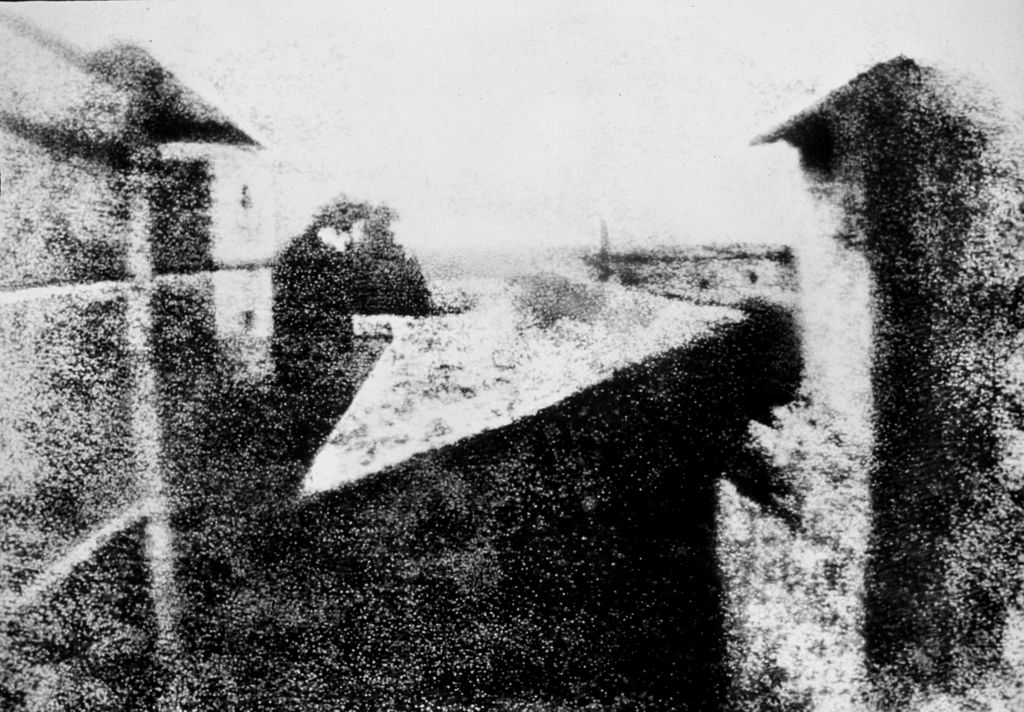
\includegraphics[width=\textwidth]{slides/graphics-introduction/first-photo.jpg}
    \textit{\small View from the Window at Le Gras picture}
  \end{minipage}
  \hfill
  \begin{minipage}[b]{0.45\textwidth}
    \centering
    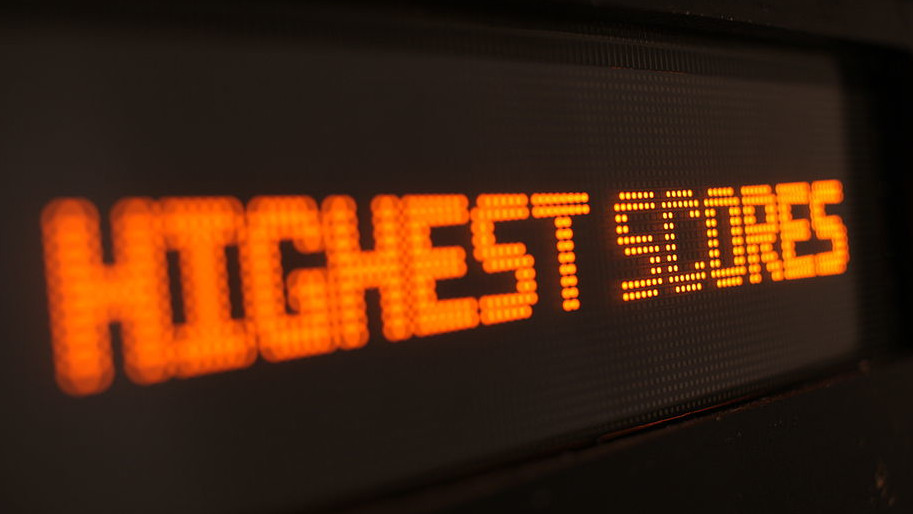
\includegraphics[width=\textwidth]{slides/graphics-introduction/dot-matrix-display.jpg}
    \textit{\small A monochrome dot-matrix display}
  \end{minipage}

  \vspace{1em}

  \begin{minipage}[b]{0.45\textwidth}
    \centering
    \textbf{Analog representation},\\ on a metal plate
  \end{minipage}
  \hfill
  \begin{minipage}[b]{0.45\textwidth}
    \centering
    \textbf{Digital representation},\\ on a LED display
  \end{minipage}
\end{frame}

\begin{frame}{Light representation, color quantization}
  \begin{minipage}[c]{0.75\textwidth}
    \begin{itemize}
    \item Light itself must be quantized in digital representations\\
    \textit{distinct from and unrelated to spatial quantization}
    \item Translating light information (colors) to numbers
    \item The translation referential is called \textbf{colorspace}
    \item The translated color has coordinates in the colorspace\\
    \textit{e.g. 3 for a human-eye-alike referential: red, green, blue}
    \item The color coordinates are quantized with:
      \begin{itemize}
      \item A given \textbf{resolution}:
      \textit{the smallest possible color difference}
      \item A given \textbf{range}:
      \textit{the span of representable colors}
      \end{itemize}
    \item Both aspects of color quantization depend on:
      \begin{itemize}
      \item The colorspace taken as referential
      \item The color depth or number of \textbf{bits per pixel} (bpp)
      \item Implementation choices
      \end{itemize}
    \end{itemize}
  \end{minipage}
  \hfill
  \begin{minipage}[c]{0.225\textwidth}
    \centering
    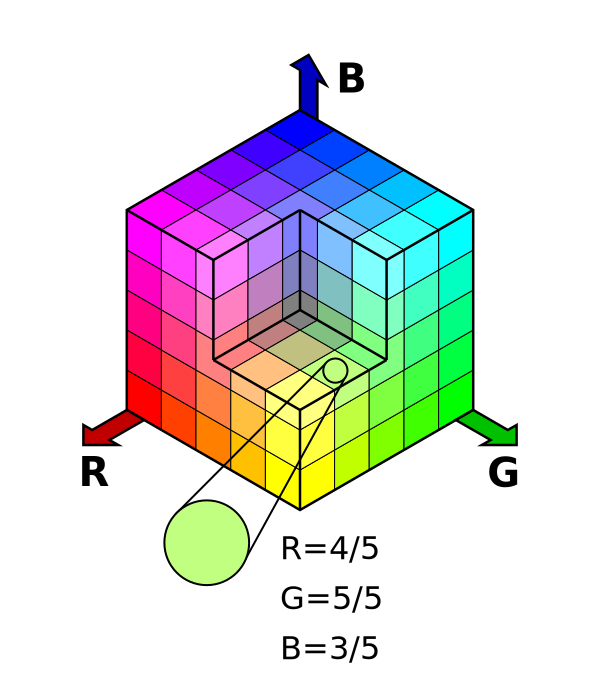
\includegraphics[width=\textwidth]{slides/graphics-introduction/rgb-cube.pdf}
  \end{minipage}
\end{frame}

\begin{frame}{Light representation, color quantization (illustrated)}
  \begin{minipage}[b]{0.45\textwidth}
    \centering
    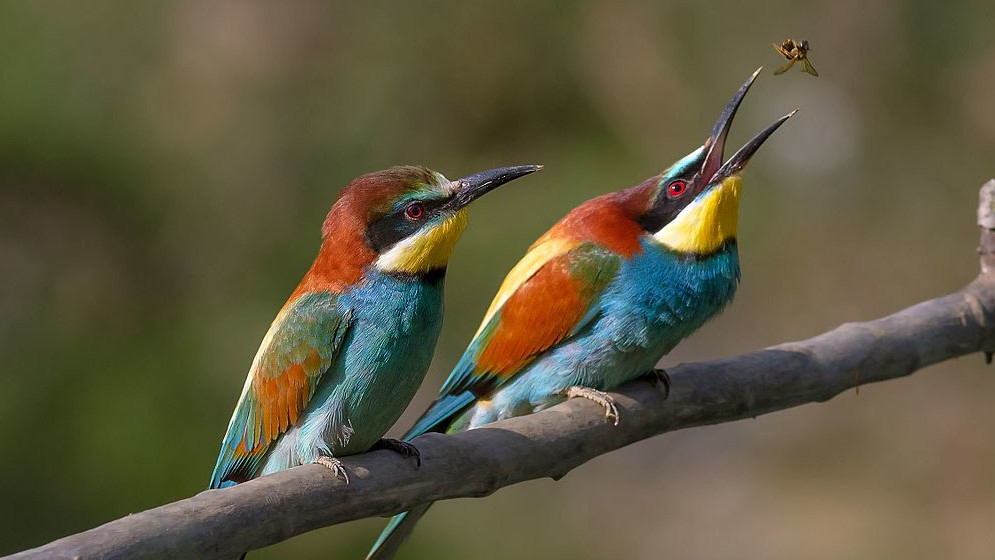
\includegraphics[width=\textwidth]{slides/graphics-introduction/pair-of-merops.jpg}
  \end{minipage}
  \hfill
  \begin{minipage}[b]{0.45\textwidth}
    \centering
    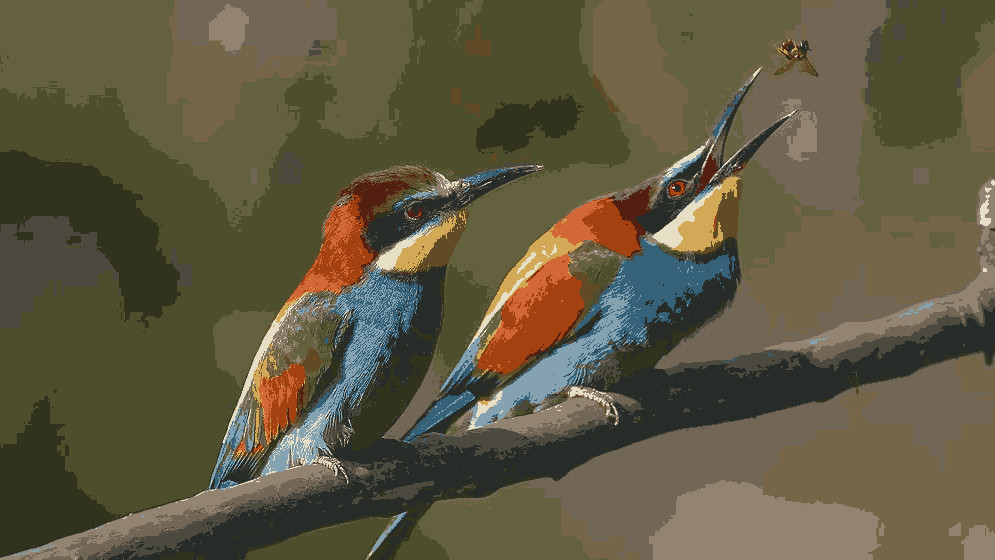
\includegraphics[width=\textwidth]{slides/graphics-introduction/pair-of-merops-16-colors.jpg}
  \end{minipage}

  \begin{center}
     \textit{\small A pair of Merops feeding}
  \end{center}

  \begin{minipage}[b]{0.45\textwidth}
    \centering
    \textbf{16 million colors (24 bits per pixel)}
    \begin{itemize}
    \item high color resolution
    \item high color range
    \end{itemize}
  \end{minipage}
  \hfill
  \begin{minipage}[b]{0.45\textwidth}
    \centering
    \textbf{16 colors (4 bits per pixel)}
    \begin{itemize}
    \item low color resolution
    \item low color range
    \end{itemize}
  \end{minipage}
\end{frame}

\begin{frame}{Light representation, color quantization (illustrated)}
  \begin{minipage}[b]{0.45\textwidth}
    \centering
    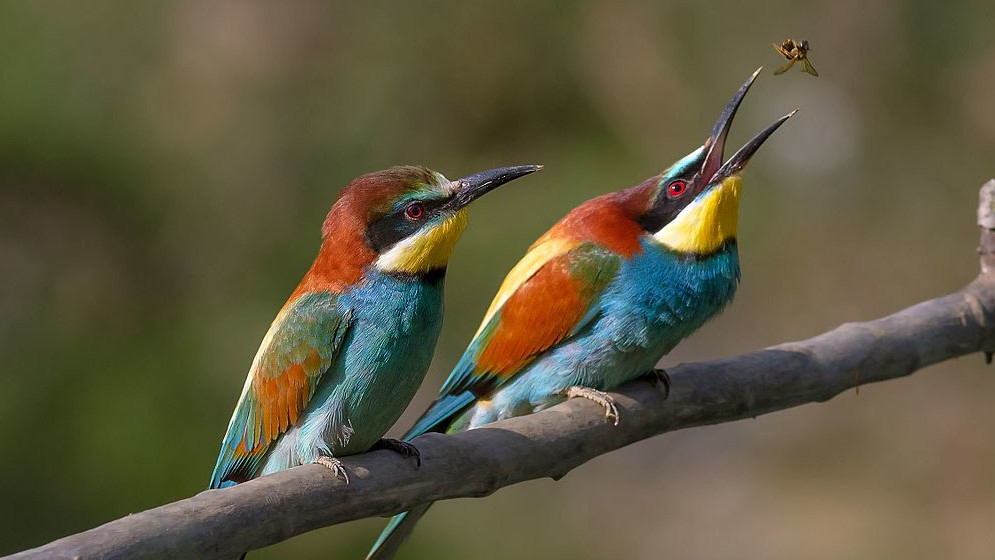
\includegraphics[width=\textwidth]{slides/graphics-introduction/pair-of-merops.jpg}
  \end{minipage}
  \hfill
  \begin{minipage}[b]{0.45\textwidth}
    \centering
    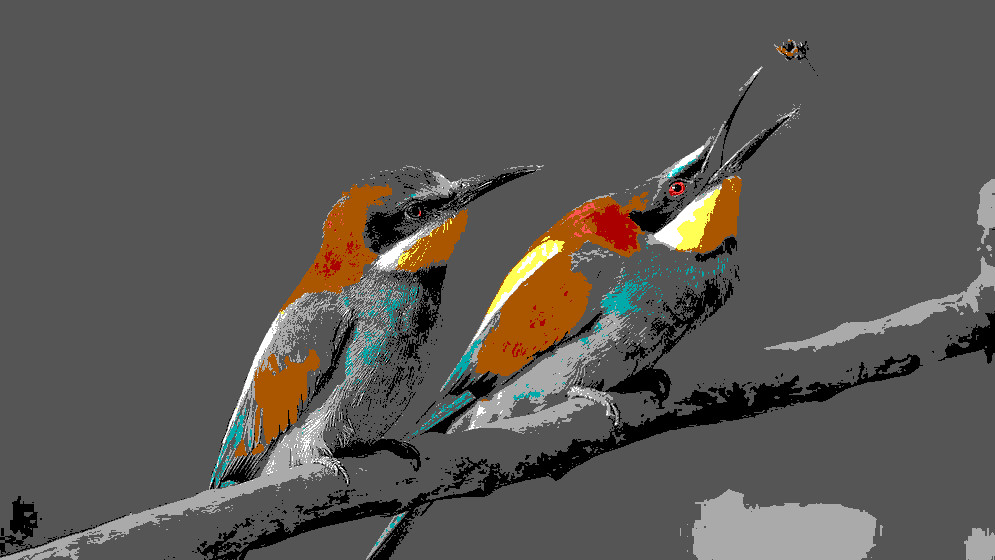
\includegraphics[width=\textwidth]{slides/graphics-introduction/pair-of-merops-16-colors-range.jpg}
  \end{minipage}

  \begin{center}
     \textit{\small A pair of Merops feeding}
  \end{center}

  \begin{minipage}[b]{0.45\textwidth}
    \centering
    \textbf{16 million colors (24 bits per pixel)}
    \begin{itemize}
    \item high color resolution
    \item high color range
    \end{itemize}
  \end{minipage}
  \hfill
  \begin{minipage}[b]{0.45\textwidth}
    \centering
    \textbf{16 colors (4 bits per pixel)}
    \begin{itemize}
    \item lower color resolution
    \item high color range
    \end{itemize}
  \end{minipage}
\end{frame}

\begin{frame}{Level of detail of quantized pictures}
  Depends on a number of factors, including:
  \begin{itemize}
  \item Spatial density (pixel resolution)
  \item Quantized dimensions (picture width and height)
  \item Colorspace limits (chromaticity diagram)
  \item Color depth (number of bits per pixel)
  \item Color resolution and range trade-off
  \end{itemize}~

  Generally speaking:
  \begin{itemize}
  \item Many factors are involved
  \item The major bottleneck is not always obvious
  \item Implementation choices do matter
  \end{itemize}
\end{frame}

\begin{frame}{Colorspaces and channels}
  \begin{minipage}[b]{0.7\textwidth}
    \begin{itemize}
    \item Each component of a colorspace is called a \textbf{channel}
    \item Examples for usual types of colorspaces:
      \begin{itemize}
      \item RGB, with 3 channels:\\ \textbf{R} (red) / \textbf{G} (green) / \textbf{B} (blue)
      \item HSV, with 3 channels:\\ \textbf{H} (hue) / \textbf{S} (saturation) / \textbf{V} (value)
      \item YUV or Y/Cb/Cr, with 3 channels:\\ \textbf{Y} (luminance) / \textbf{U or Cb} / \textbf{V or Cr} (chrominance)
      \end{itemize}
    \end{itemize}
  \end{minipage}
  \hfill
  \begin{minipage}[b]{0.25\textwidth}
    \centering
    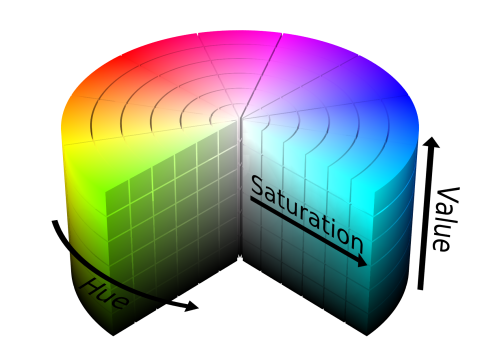
\includegraphics[width=\textwidth]{slides/graphics-introduction/hsv-diagram.pdf}\\
    \vspace{-1em}
    \textit{\small HSV diagram}
    \vspace{0.25em}
  \end{minipage}
  \begin{itemize}
  \item An additional channel can exist for transparency: the \textbf{alpha channel}\\
  \textit{mostly relevant for composition, not for final display}
  \item Color coordinates can be \textbf{converted} from one colorspace to another (CSC)\\
  \textit{using translation formulas and associated constants}
  \end{itemize}
\end{frame}

\begin{frame}{Colorspaces and channels (illustrated with YUV)}
  \begin{minipage}[t]{0.25\textwidth}
    \centering
    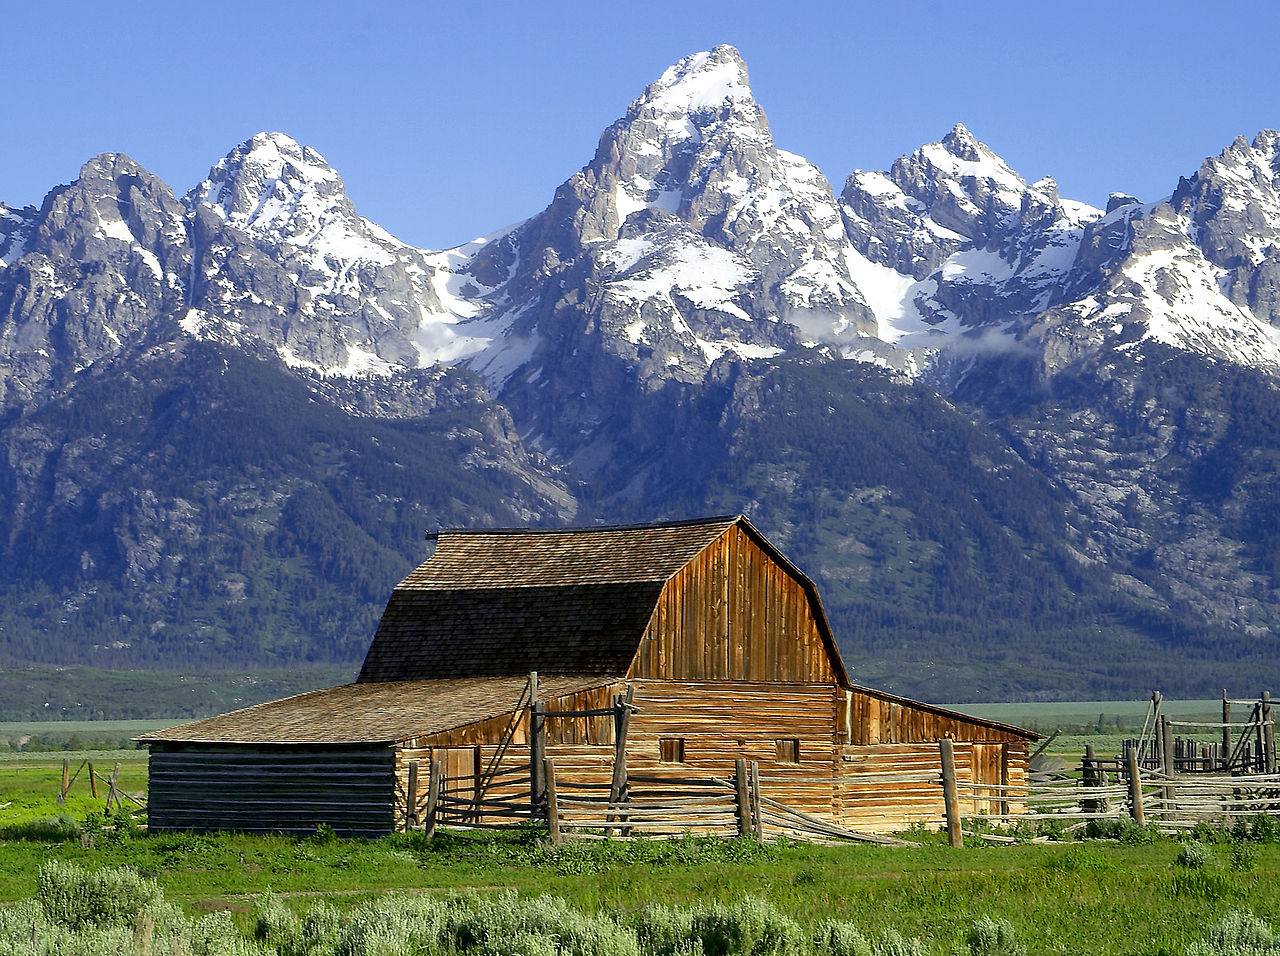
\includegraphics[height=6em]{slides/graphics-introduction/barn.jpg}\\
    \textit{\small Original picture}
  \end{minipage}
  \hfill
  \begin{minipage}[t]{0.7\textwidth}
    \centering
    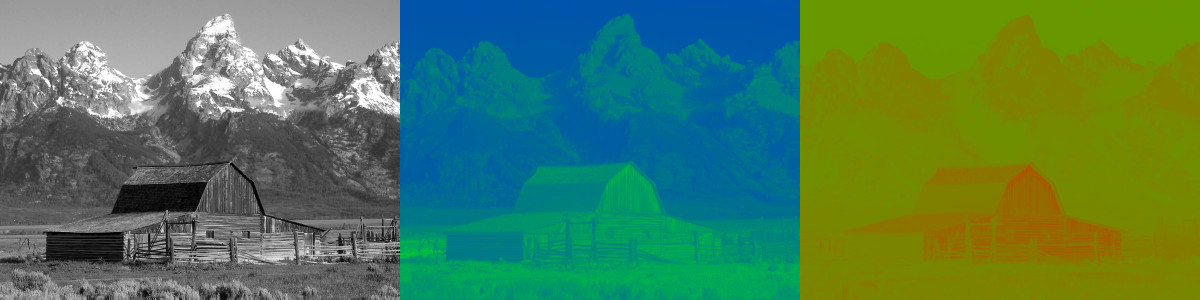
\includegraphics[height=6em]{slides/graphics-introduction/barn-yuv.jpg}\\
    \textit{\small Decomposition in Y, U and V channels}
  \end{minipage}

  \vspace{1em}

  \begin{minipage}[t]{0.4\textwidth}
    \small
    \begin{equation*}
    \begin{cases}
    R = Y + 1.140 \times V\\
    G = Y - 0.395 \times U - 0.581 \times V\\
    B = Y + 2.032 \times U
    \end{cases}
    \end{equation*}
  \end{minipage}
  \hfill
  \begin{minipage}[t]{0.55\textwidth}
    \small
    \begin{equation*}
    \begin{cases}
    Y = + 0.299 \times R + 0.587 \times G + 0.114 \times B\\
    U = - 0.147 \times R - 0.289 \times G + 0.436 \times B\\
    V = + 0.615 \times R - 0.515 \times G - 0.100 \times B
    \end{cases}
    \end{equation*}
  \end{minipage}

  \begin{center}
     \textit{\small Translation between BT.609 YUV and sRGB colorspaces}
  \end{center}
\end{frame}

\begin{frame}{Frame size and chroma sub-sampling}
  \begin{itemize}
  \item Digital pictures easily take up a lot of space (moreso for videos)
  \item The minimal size for a picture depends on:
    \begin{itemize}
    \item Dimensions (\(width\) and \(height\))
    \item Color (and alpha) depth or bits per pixel (\(bpp\))
    \item Roughly: \(width \times height \times bpp \div 8~bytes\)
    \item For 12 Mpixels with 16 Mcolors and alpha: \(4000 \times 3000 \times 32 \div 8 = 45.8 MiB\)
    \end{itemize}
  \item The human visual system has specificities:
    \begin{itemize}
    \item High sensitivity to \textbf{luminosity} (luminance)
    \item Low sensibility to \textbf{colors} (chrominance)
    \end{itemize}
  \item YUV colorspaces offer the relevant channel separation
  \item Sub-sampling can be applied to the chrominance channel\\
  \textit{less data (and precision) on colors to reduce size}
  \end{itemize}
\end{frame}

\begin{frame}{Frame size and chroma sub-sampling}
  \begin{itemize}
  \item Chrominance samples are used for multiple luminance samples
  \item With specific vertical and horizontal ratios (usually integer)
  \item Usually summarized using a three-part ratio: \(J:a:b\)
  \end{itemize}

  \begin{center}
  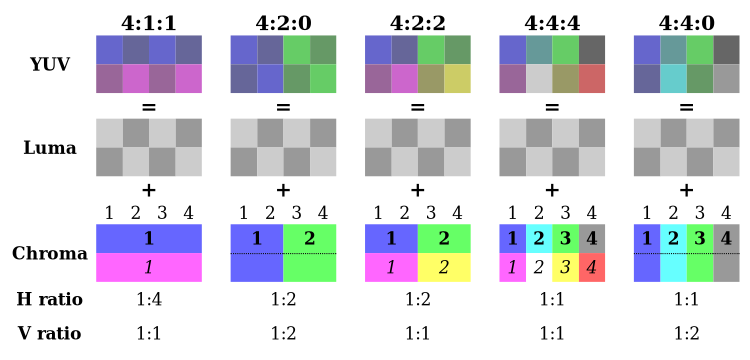
\includegraphics[width=0.7\textwidth]{slides/graphics-introduction/yuv-sub-sampling.pdf}

  YUV 4:2:0 usual example:\\
  {\small\(bpp_Y = 8,~bpp_U = 8 / 2 = 4,~bpp_V = 8 / 2 = 4 ~\Rightarrow~ bpp = 16~bits/pixel\)}
  \end{center}
\end{frame}

\begin{frame}[fragile]{Pixel formats, FourCC codes}

  \begin{itemize}
  \item Many meta-data elements are needed to fully describe how a picture is coded
    \begin{itemize}
    \item Some describe \textbf{picture-level attributes} (e.g. dimensions)
    \item Some describe \textbf{pixel-level attributes} (e.g. colorspace, bpp)
    \end{itemize}
  \item Picture-level attributes are kept
  \item Pixel-level attributes are grouped as a \textbf{pixel format}
  \item Pixel formats precisely define how pixels are represented:
    \begin{itemize}
    \item Colorspace in use
    \item Number of bits per channel and per pixel (bpp)
    \item Bit attribution and endianness
    \item Per-channel sub-sampling ratios
    \end{itemize}
  \item Often represented as a 4-character code called \textbf{FourCC} {\small(\url{https://fourcc.org/})}\\
  \textit{Not really standardized but widely used in various forms}
  \item Example: \verb,DRM_FORMAT_XRGB8888, is defined with the \verb,XR24, FourCC
  \end{itemize}

\end{frame}

\subsection{Basic Drawing and Processing}

\begin{frame}{Ideas}

* how to draw pixels (XRGB32)
* iterating a frame's pixels (h > w)
* 

\end{frame}

\subsection{Advanced Processing}

\section{Hardware Aspects}

\subsection{Pipeline Components Overview and Generalities}

\begin{frame}{Technological types of graphics hardware implementations}
  \begin{itemize}
  \item Two commonly-used technologies, specific pros/cons:
  \end{itemize}

  \begin{center}
  \small
  \def\arraystretch{1.2}
  \begin{tabular}{l|c|c}
  & \textbf{Fixed-function} & \textbf{Programmable} \\
  \hline
  \textbf{Technology} & Circuit & Software \\
  \textbf{Source form} & HDL & Source code \\
  \textbf{Product form} & Silicon, bitstream & Firmware binaries \\
  \textbf{Implementation medium} & FPGA, ASIC, SoC block & DSP, custom ISA \\
  \textbf{Arithmetic} & Fixed-point & Fixed-point, floating point \\
  \textbf{Clock rate} & Low & High \\
  \textbf{Pixel data access} & Queue (FIFO) & Memory \\
  \textbf{CPU control} & Direct registers & Mailbox \\
  \textbf{Die surface (tendency)} & High & Low \\
  \textbf{Reusability} & Low & High \\
  \hline
  \textbf{Example} & Allwinner SoCs Display Engine & TI TMS340 DSP \\
  \end{tabular}
  \end{center}
\end{frame}

\begin{frame}{Graphics memory and buffers}
  \begin{itemize}
  \item Pixel data is stored in memory buffers, called \textbf{framebuffers}
  \item Framebuffers live either on:
    \begin{itemize}
    \item \textbf{System memory}: shared with the rest of the system (e.g. SDRAM or SRAM)
    \item \textbf{Dedicated memory}: only for graphics (e.g. SGRAM)
    \end{itemize}
  \item Framebuffers that can be displayed are called \textbf{scanout framebuffers}\\
  \textit{hardware constraints don't always allow any framebuffer to be scanned out}
  \item CPU access to pixel data in dedicated memory is not always granted or easy!
  \item Graphics hardware \textbf{needs configuration} to interpret framebuffer pixel data\\
    \textit{pixel meta-data is rarely to never stored aside of the pixel data}
  \end{itemize}
\end{frame}

\begin{frame}{I/O with graphics hardware, pipelines}
  \begin{itemize}
  \item Graphics hardware is \textbf{I/O-based} and interacts with pixel data
  \item Pipeline elements have input-output abilities:
    \begin{itemize}
    \item \textbf{Source} components: \textbf{feed pixel data}: \textit{e.g. camera}
    \item \textbf{Sink} components: \textbf{grab pixel data}: \textit{e.g. display}
    \end{itemize}
  \item Some components are \textbf{both a source and a sink}: \textit{e.g. converters}
  \item Graphics components can be chained in \textbf{pipelines}\\
    \textit{Usually from a source-only element to a sink-only element}
  \end{itemize}

  \vspace{-2em}
  \begin{center}
  \includegraphics[width=0.7\textwidth]{slides/graphics-introduction/pipeline-sink-source.pdf}
  \end{center}
\end{frame}

\begin{frame}{Display hardware overview}
  \begin{itemize}
  \item \textbf{Stream pixel data} to a display device, via a display interface
  \item Internal pipeline with \textbf{multiple components}
  \item Generally \textbf{fixed-function} hardware, pipeline sink only
  \item Either \textbf{discrete} (video card) or \textbf{integrated}
  \item Connected to the CPU (and RAM) via a \textbf{high-speed bus}:\\
  \textit{e.g. AXI with ARM, ISA, PCI, AGP, PCI-e with x86}
  \end{itemize}~

  \begin{minipage}[t]{0.45\textwidth}
    \centering
    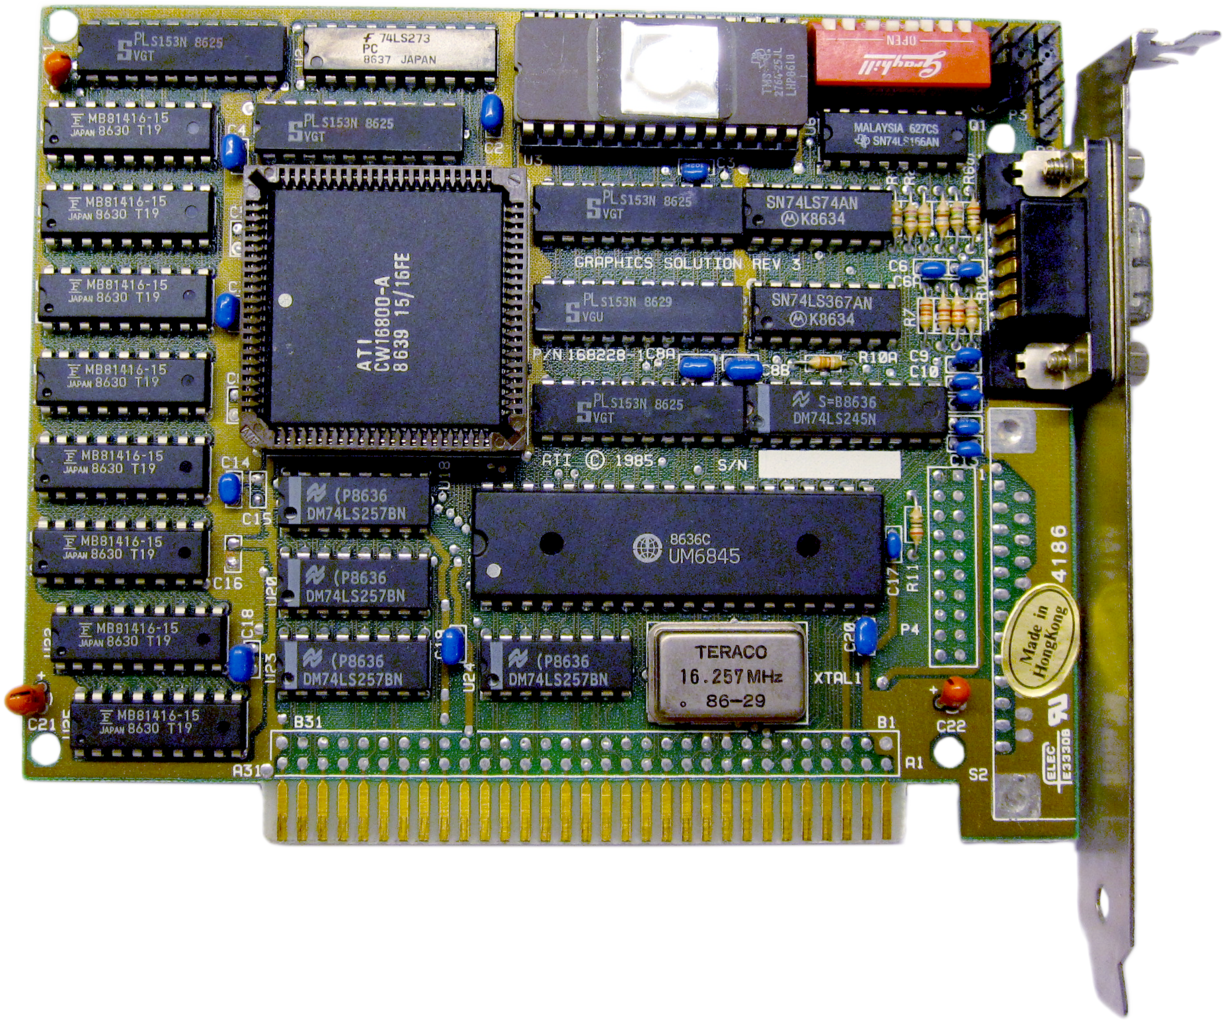
\includegraphics[height=7em]{slides/graphics-introduction/ati-hercules-1986.png}\\
    \textit{\small A 1986 Hercules discrete video card}
  \end{minipage}
  \hfill
  \begin{minipage}[t]{0.45\textwidth}
    \centering
    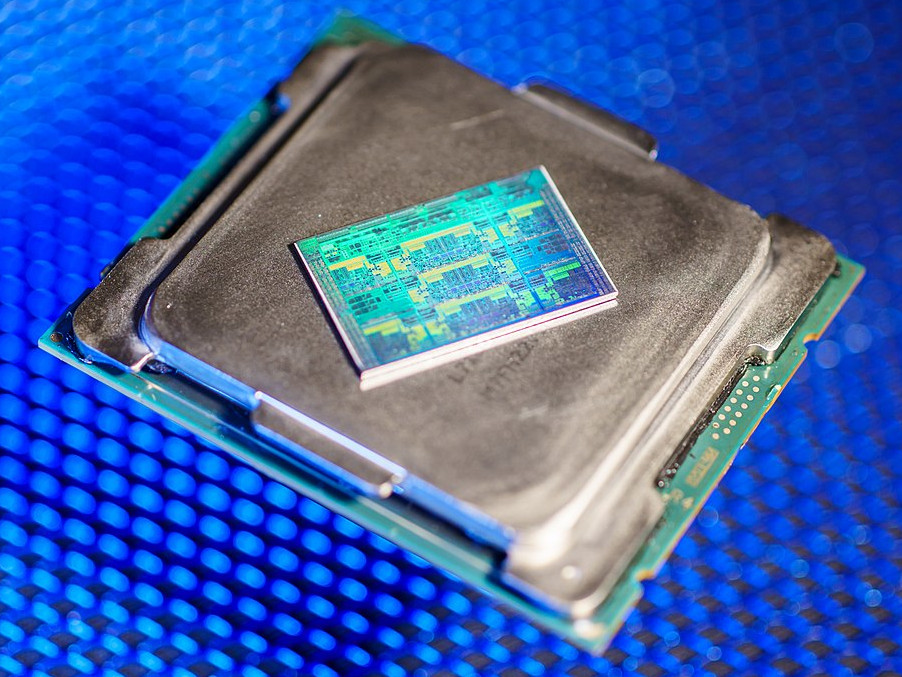
\includegraphics[height=7em]{slides/graphics-introduction/intel-skylake.jpg}\\
    \textit{\small An Intel processor with integrated graphics}
  \end{minipage}
\end{frame}

\begin{frame}{Common components of a display pipeline overview}
  \begin{center}
  \includegraphics[width=0.7\textwidth]{slides/graphics-introduction/display-pipe.pdf}
  \end{center}

  \begin{enumerate}
  \item \textbf{Framebuffers} where the pixel data is stored
  \item \textbf{Planes} that associate a framebuffer with its dimensions and position
  \item \textbf{CRTC} for pixel composition and streaming\\
  \textit{The CRTC terminology comes from the legacy Cathode-Ray Tube Controller}
  \item \textbf{Encoder} for meta-data addition and physical signal conversion
  \item \textbf{Connector} for video signal, display data channel (DDC), hotplug detection
  \item \textbf{Monitor} for decoding and displaying pixels (decoder and panel)
  \end{enumerate}
\end{frame}

\begin{frame}{Rendering hardware overview}
  \textbf{Rendering} hardware includes a wide range of aspects (usual cases below):
  \begin{itemize}
  \item \textbf{Basic} pixel processing:
  \begin{itemize}
    \item Common operations: pixel format, CSC, dithering, scaling, blitting and blending
    \item Fixed-function hardware, pipeline sink and source
  \end{itemize}
  \item \textbf{Complex} pixel processing:
  \begin{itemize}
    \item Defined by the application: any computable operation
    \item Programmable hardware (DSP), pipeline sink and source
  \end{itemize}
  \item \textbf{2D vector} drawing:
  \begin{itemize}
    \item From equations, parameters and data (e.g. points)
    \item Either fixed-function or programmable hardware (custom), pipeline source
  \end{itemize}
  \item \textbf{3D scene} rendering:
  \begin{itemize}
    \item From programs (shaders) and data (e.g. vertices, textures)
    \item Programmable hardware (GPU), pipeline source
  \end{itemize}
  \item Rendering can \textbf{always fallback} to general-purpose CPU operations
  \end{itemize}
\end{frame}

\begin{frame}{Video hardware overview}
  \textbf{Video-oriented} hardware comes in different forms (usual cases below):

  \begin{itemize}
  \item \textbf{Hardware video decoder} (VPU/video codec decoder)
  \begin{itemize}
    \item Decodes a video from compressed data (bitstream) to pixel frames
    \item Fixed-function hardware, pipeline source
  \end{itemize}
  \item \textbf{Hardware video encoder} (VPU/video codec encoder)
  \begin{itemize}
    \item Encodes a video from pixel frames to compressed data (bitstream)
    \item Fixed-function hardware, pipeline sink
  \end{itemize}
  \item \textbf{Camera sensors, video input, video broadcasting} (DVB)
  \begin{itemize}
    \item Receives/sends data in a given configuration from/to \textit{the outside}
    \item Can be compressed data (bitstream) or raw pixel data
    \item Fixed-function hardware, pipeline source
  \end{itemize}
  \end{itemize}~
\end{frame}

\begin{frame}{Building complex pipelines}

  \begin{itemize}
  \item Display, rendering and video elements are chained from source(s) to sink(s)
  \item On source-sink boundaries:
    \begin{itemize}
    \item Mutually-supported pixel format (or conversion)
    \item Mutually-accessible memory (or copy)
    \end{itemize}
  \item Target frame rate (\(fps\)) gives a time budget for pipeline traversal:
  \( t_0 + t_2 + t_4 + t_5 < fps^{-1},~ t_0 + t_3 < fps^{-1},~ t_1 + t_4 + t_5 < fps^{-1} \)
  \end{itemize}

  \begin{center}
  \includegraphics[width=0.7\textwidth]{slides/graphics-introduction/pipeline-complex.pdf}
  \end{center}

\end{frame}

\subsection{Display Hardware Specifics}

\begin{frame}{Visual display technologies generalities}
  \begin{itemize}
  \item Pixel data is pushed from the display interface to a visible surface\\
  \textit{using a dedicated controller on the display device}
  \item Pixels are split into 3 color cells (R-G-B)
  \item The human eye naturally merges light from the 3 cells
  \item Pixel frames are displayed as (physical) arrays of color cells
  \end{itemize}~

  \begin{minipage}[b]{0.45\textwidth}
    \centering
    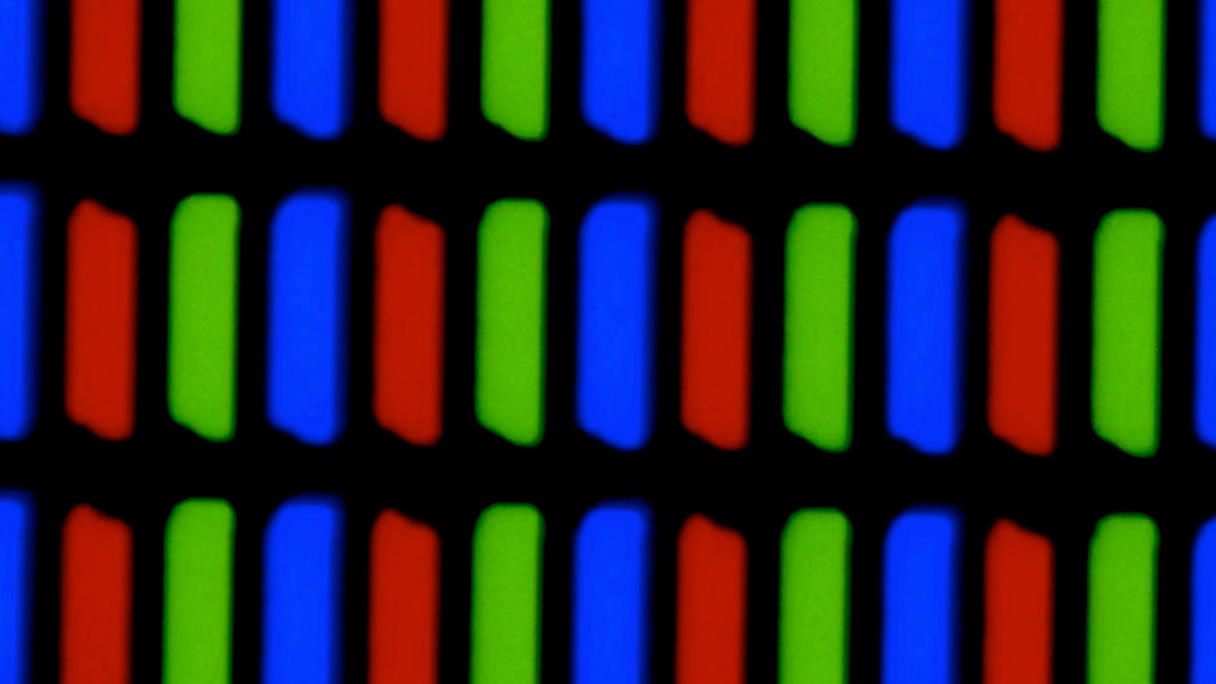
\includegraphics[height=6.5em]{slides/graphics-introduction/pixel-array.jpg}\\
    \textit{\small Pixel color cells on a LCD TN panel}
  \end{minipage}
  \hfill
  \begin{minipage}[b]{0.45\textwidth}
    \centering
    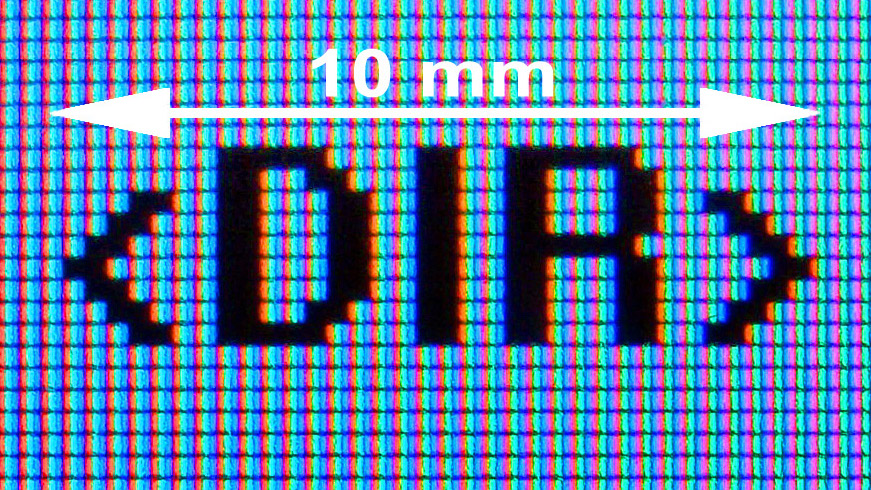
\includegraphics[height=6.5em]{slides/graphics-introduction/pixel-array-text.jpg}\\
    \textit{\small A pixel array displaying text}
  \end{minipage}
\end{frame}

\begin{frame}{CRT display technology}
  \begin{itemize}
  \item Color \textbf{cathode-ray tubes} (CRTs), since the 1950s:
    \begin{itemize}
    \item Using electron beams to excite a phosphorescent screen
    \item Beams are guided by magnetic deflection
    \item One beam for each color with increased intensity for increased luminosity
    \item High energy consumption
    \item High contrast, medium response time (\(1-10~\mu s\))
    \item Other issues: monitor size, burn-in (screensavers), remanent magnetic field (degaussing), high voltages and magnetic fields
    \end{itemize}
  \end{itemize}

  \begin{center}
  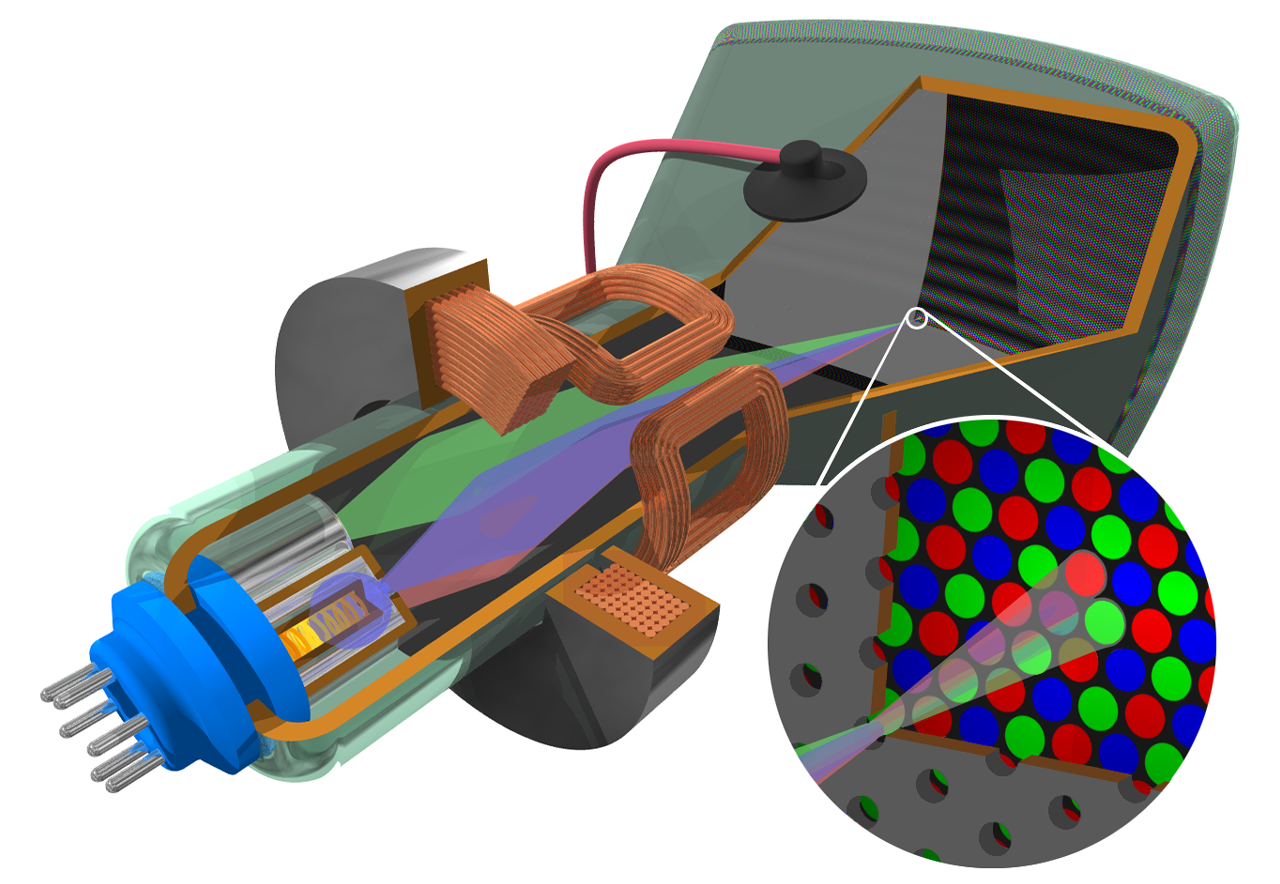
\includegraphics[height=8em]{slides/graphics-introduction/crt-color.png}
  \end{center}
\end{frame}

\begin{frame}{Plasma display panels technology}
  \begin{itemize}
  \item \textbf{Plasma display panels} (PDPs), since the 1990s-2000s:
    \begin{itemize}
    \item Using gas cells brought to plasma state to strike light-emitting phosphor
    \item Flat array of cells, scales to large surfaces
    \item Medium energy consumption (depends on luminance)
    \item Medium to low contrast, low response time (\(\leq 1~\mu s\))
    \item Other issues: burn-in
    \item Gradually being \textbf{deprecated} in favor of other flat-panel technologies
    \end{itemize}
  \end{itemize}
\end{frame}

\begin{frame}{LCD display technology}
  \begin{itemize}
  \item \textbf{Liquid crystal displays} (LCDs) using \textbf{Thin-film-transistors} (TFT):
    \begin{itemize}
    \item Using the electrically-controlled alignment of crystal structures to block light
    \item Does not emit light: needs an always-on backlight source (usually LEDs)
    \item Low energy consumption (depends on backlight)
    \item Medium to low contrast, high response time (\(1-10~ms\))
    \item \textbf{Twisted nematic} (TN): limited color quality and viewing angles, since the 1980s
    \item \textbf{In-plane switching} (IPS): improved color and viewing angles, since the 2000s
    \end{itemize}
  \end{itemize}

  \begin{center}
  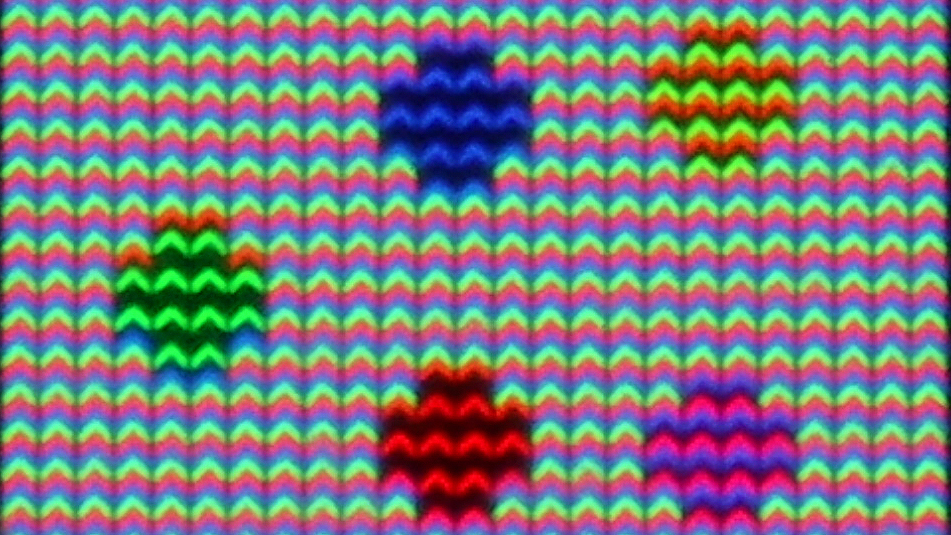
\includegraphics[height=6em]{slides/graphics-introduction/lcd-ips-shape.jpg}\\
  \textit{\small Chevron shapes that improve the viewing angle on IPS LCDs}
  \end{center}
\end{frame}

\begin{frame}{OLED display technology}
  \begin{itemize}
  \item \textbf{Organic light-emitting diodes} (OLEDs), since 2010:
    \begin{itemize}
    \item Using organic compounds (carbon-based) to emit light as R-G-B LEDs
    \item Allows flat and flexible surfaces, with a large viewing angle
    \item Low energy consumption
    \item Very high contrast, high response time (\(1-10~\mu s\))
    \item Issues: burn-in, independent cells aging, affected by UV light
    \item Rapidly becoming \textbf{very popular} and used
    \end{itemize}
  \end{itemize}

  \begin{center}
  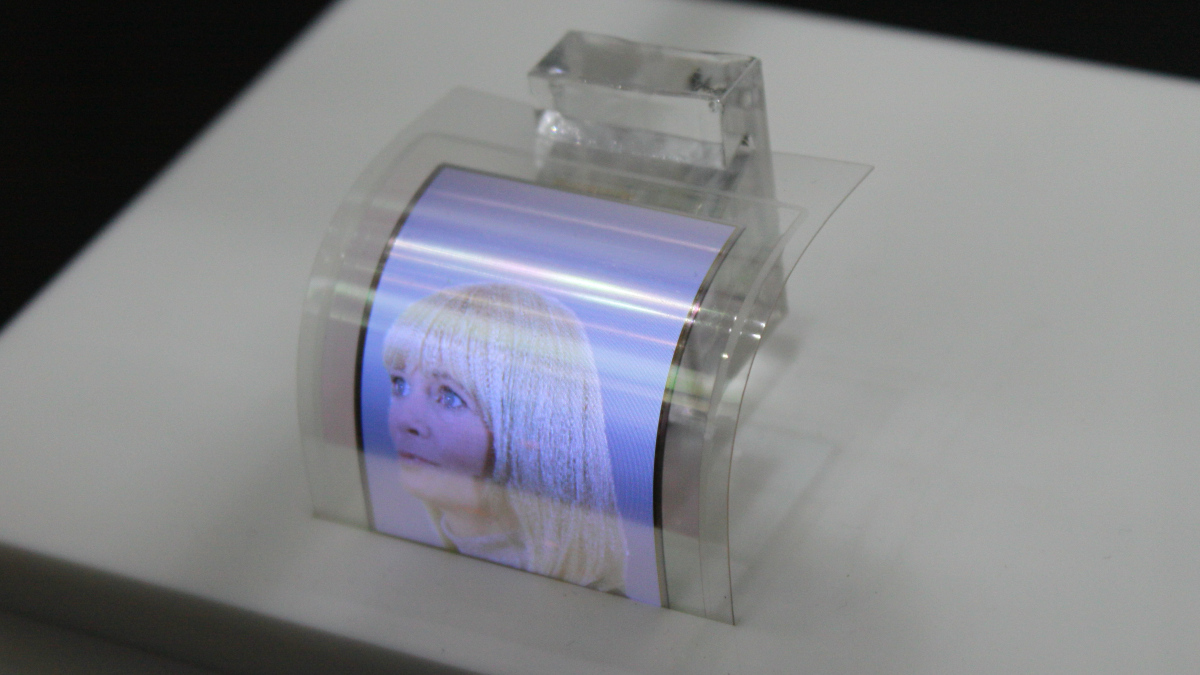
\includegraphics[height=8em]{slides/graphics-introduction/oled-display.jpg}\\
  \textit{\small A flexible OLED display panel}
  \end{center}
\end{frame}

\begin{frame}{EPD display technology}
  \begin{itemize}
  \item \textbf{Electrophoretic displays} (EPDs), since the 2000s:
    \begin{itemize}
    \item Using black and white electrically-charged particles in ink\\
    \textit{e.g. positive charge for black and negative for black}
    \item Electric fields attract one or the other color with current flow
    \textit{the particles stay in place after they were moved}
    \item Using incident light, does not emit light itself
    \item Very low consumption (only for changes)
    \item Low response time (\(1-10~\mu s\)) and ghosting
    \end{itemize}
  \end{itemize}~

  \begin{minipage}[b]{0.45\textwidth}
    \centering
    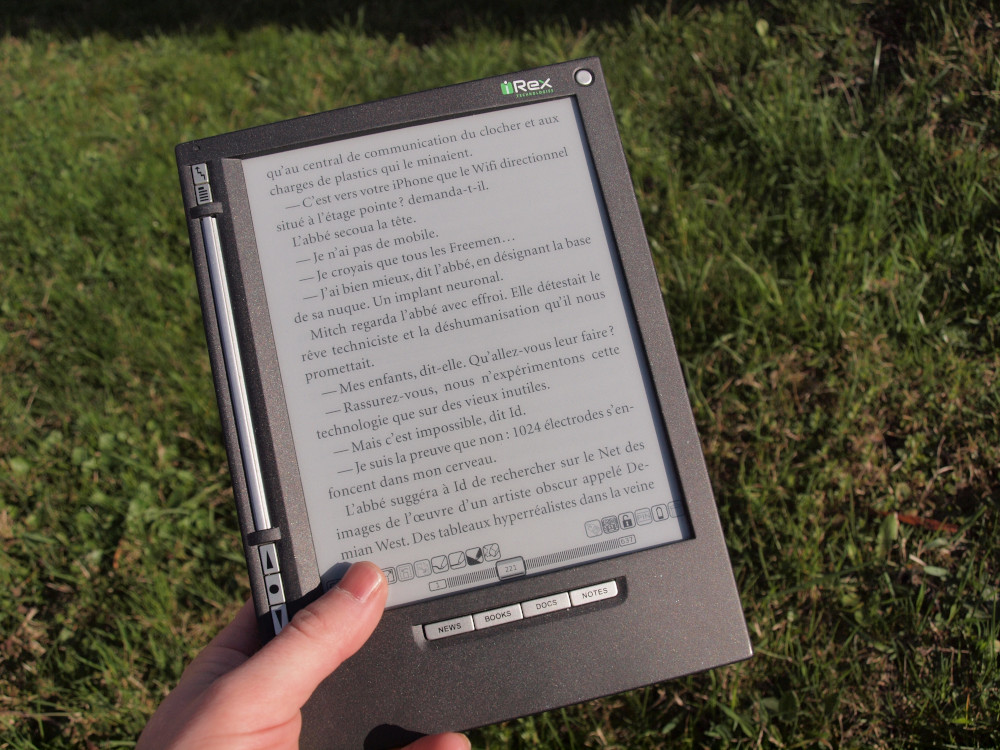
\includegraphics[height=6.5em]{slides/graphics-introduction/e-reader.jpg}\\
    \textit{\small An e-reader with an EPD display}
  \end{minipage}
  \hfill
  \begin{minipage}[b]{0.45\textwidth}
    \centering
    
\includegraphics[height=6.5em]{slides/graphics-introduction/epd-detail.jpg}\\
    \textit{\small Detail of an EPD display}
  \end{minipage}
\end{frame}

\begin{frame}{CRTs, refreshing and timings}
  \begin{itemize}
  \item CRTs need frequent refreshing or the picture fades out: \textbf{fixed refresh rate}
  \item An electron gun aims for pixels in \textbf{row-major/raster order}\\
  \textit{left to right from top to bottom order}
  \item Some \textbf{blank time} is needed to reposition the gun (horizontally and vertically)
  \item As a result, \textbf{specific timings} are needed for the signals to each CRT display
  \item For backwards compatibility with CRTs, \textbf{display timings are still necessary}\\
    \textit{(even when the display is really not a CRT)}
  \end{itemize}
\end{frame}

\begin{frame}{Display timings and modes}
  \begin{itemize}
  \item Timings coordinate how a frame is \textbf{transmitted to a display over time}
  \item Various signals are involved, synced to a \textbf{pixel clock} (time base)
  \item Display timings are split in a few stages (horizontal and vertical):
    \begin{enumerate}
    \item Sync pulse (vsync/hsync)
    \item Back porch (vbp/hbp)
    \item Active region (vactive/hactive)
    \item Front porch (vfp/hfp)
    \end{enumerate}
  \item Pixels are transmitted during the \textbf{horizontal active region} only
  \item A \textbf{display mode} groups timings, refresh rate and associated pixel clock rate
  \item Display signals are \textbf{generated by the CRTC}, according to the display mode
  \item Monitors usually support \textbf{multiple modes} (and dimensions)
  \end{itemize}
\end{frame}

\begin{frame}{Display timings and modes (illustrated)}
  \begin{center}
  \includegraphics[width=0.8\textwidth]{slides/graphics-introduction/display-timings.pdf}
  \end{center}

  \begin{itemize}
  \item The unit for horizontal stages is \textbf{one pixel clock period}
  \item The unit for vertical stages is \textbf{one line's duration}
  \end{itemize}
\end{frame}

\begin{frame}{Display timings and modes (panel example)}

  \begin{minipage}[b]{0.35\textwidth}
    \centering
    \vspace{2em}
    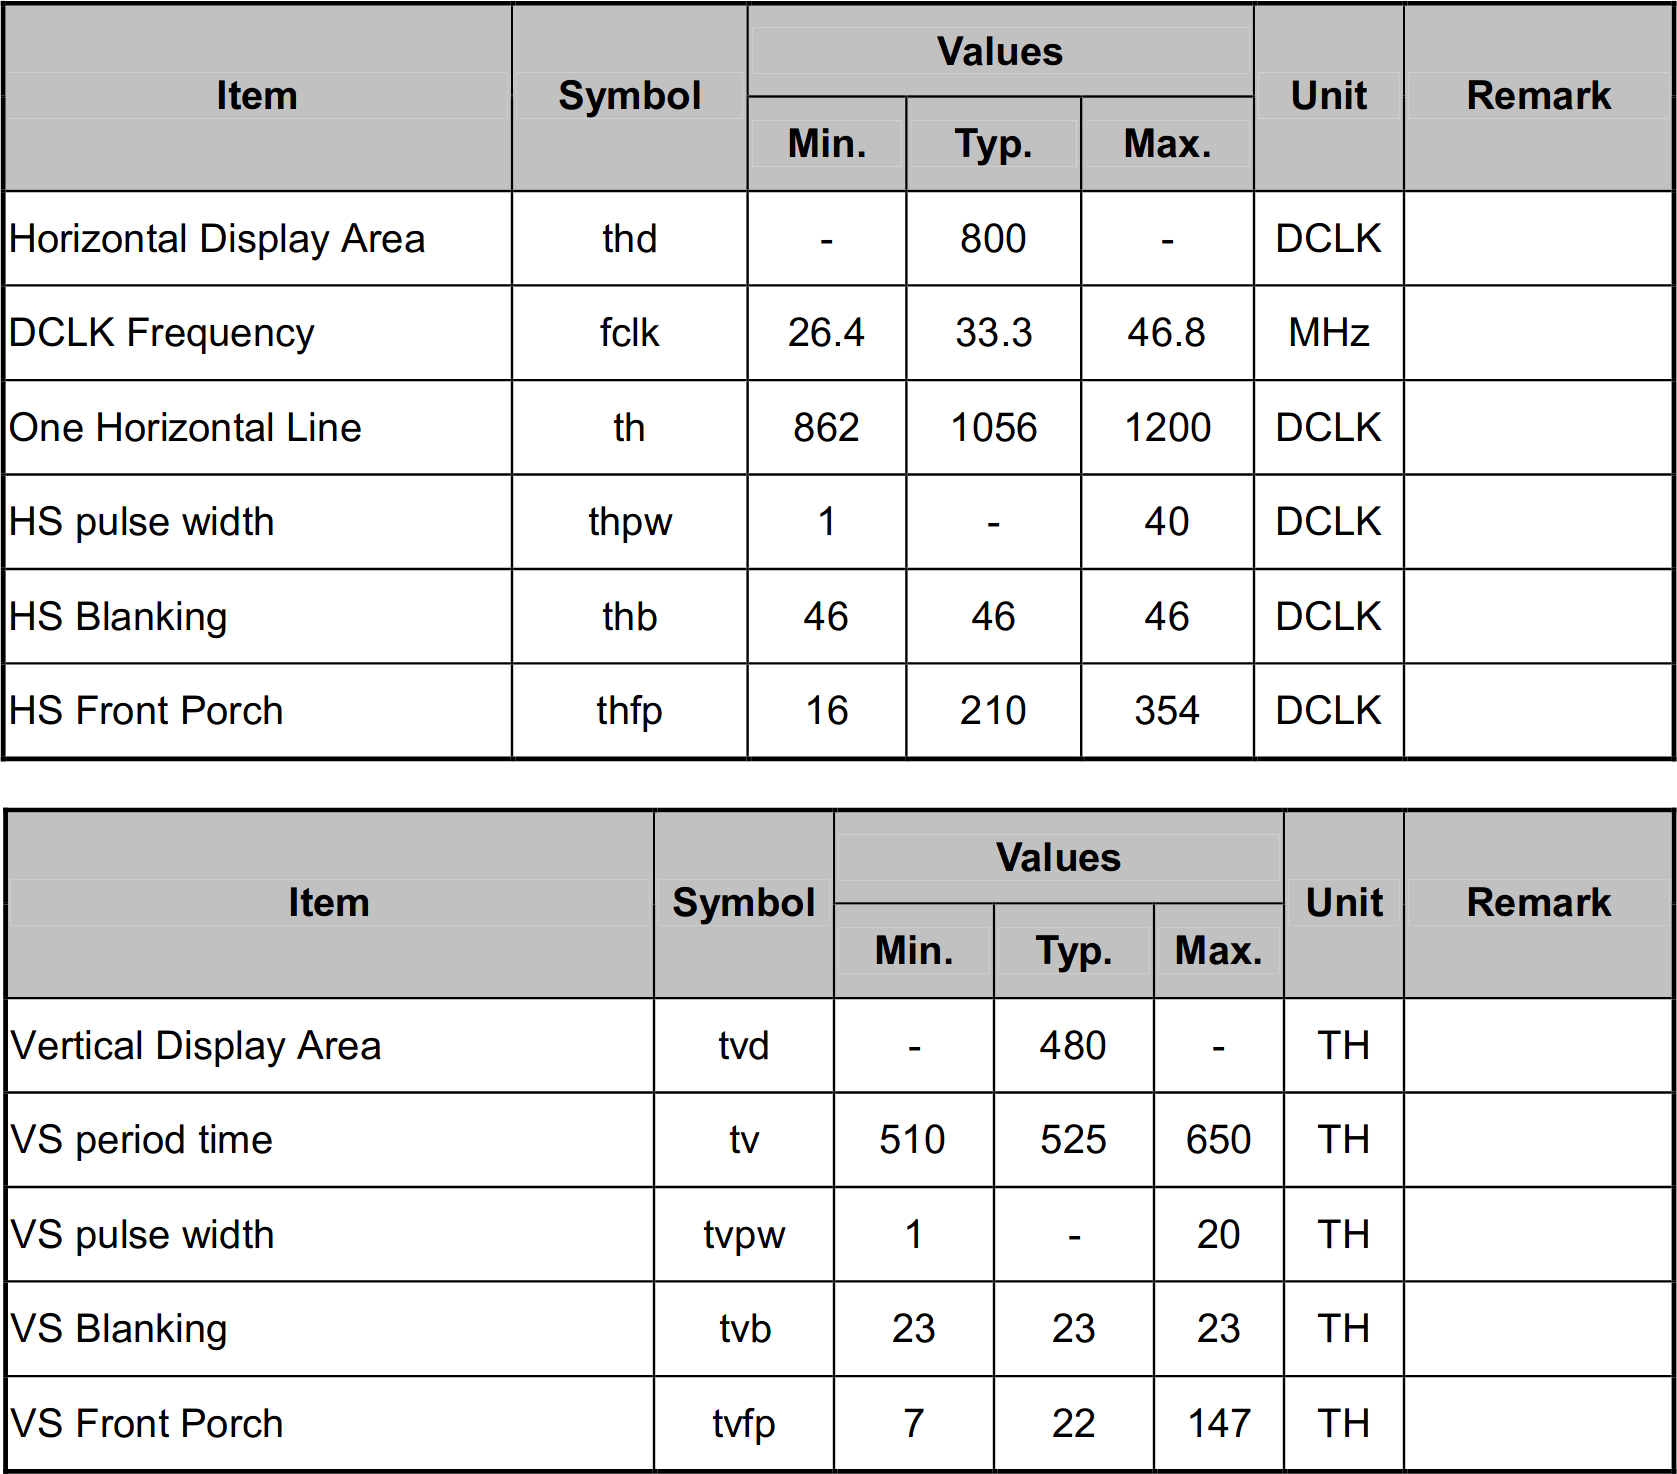
\includegraphics[width=\textwidth]{slides/graphics-introduction/timings-table.png}
    \textit{\small AT070TN94 panel datasheet}
    \vfill~
  \end{minipage}
  \hfill
  \begin{minipage}[b]{0.6\textwidth}
    \small
    \begin{itemize}
    \item \(hsync = thpw = 20 \in \llbracket 1;40 \rrbracket\)\\
    \(hbp = thb - thpw = 46 - 20 = 26\) (from diagram)\\
    \(hactive = thd = 800\)\\
    \(hfp = thfp = 210 \in \llbracket 16;354 \rrbracket\)\\
    \(htotal = hsync + hbp + hactive + hfp = 1056\)

    \item \(vsync = tvpw = 10 \in \llbracket 1;20 \rrbracket\)\\
    \(vbp = tvb - tvpw = 23 - 10 = 13\) (from diagram)\\
    \(vactive = tvd = 480\)\\
    \(vfp = tvfp = 22 \in \llbracket 7;147 \rrbracket\)\\
    \(vtotal = vsync + vbp + vactive + vfp = 525\)
    \item 1 frame takes: \(vtotal \times htotal = 554400~t_{clk}\)\\
    60 frames take: \(vtotal \times htotal \times 60 = 33264000~t_{clk}\)\\
    60 fps requires: \(f_{clk} \geq 33.264~MHz\)
    \end{itemize}
  \end{minipage}
  \vspace{0.5em}

  \begin{itemize}
  \item Panels usually support a \textbf{range of timings}
  \item The pixel clock rate is often \textbf{rounded} (refresh rate not always strictly respected)
  \end{itemize}

\end{frame}

\begin{frame}{Side-channel and identification}
  \begin{itemize}
  \item Monitor display connectors often come with a \textbf{Display Data Channel} (DDC)
    \begin{itemize}
    \item Side-bus to allow communication between host and display
    \item Usually based on I2C, quite slow (\(\approx 100~kHz\))
    \end{itemize}
  \item DDC provides access to the \textbf{Extended Display Identification Data} (EDID)
    \begin{itemize}
    \item Contains the list of supported modes in a standard format
    \item Usually stored in an EEPROM at I2C address \(0x50\)
    \end{itemize}
  \item Another common monitor signal is \textbf{Hotplug Detect} (HPD)
    \begin{itemize}
    \item Connected to a pin of the connector, asserted with a cable plugged
    \item Can be wired to an interrupt pin to detect connection changes
    \end{itemize}
  \item Direct panel interfaces (not monitors) usually lack DDC, EDID and HPD
    \begin{itemize}
      \item Panel is always considered connected
      \item Modes need to be known in advance
    \end{itemize}
  \end{itemize}
\end{frame}

\begin{frame}{Extra display interface features and EDID extensions}
  \begin{itemize}
  \item The EDID standard keeps evolving and exposes new features through extensions
  \item Configuration data for each feature is embedded in the EDID
  \item More or less features are supported depending on the display interface
  \item Common extra display interface features:
    \begin{itemize}
    \item \textbf{Interlaced}: Every other pixel line is sent at a time, alternating between top-fields and bottom-fields; Allows faster refreshing for CRTs, needs deinterlacing for progressive panels;
    \item \textbf{Audio}: Send audio in addition to pixels, during blanking periods;
    \item \textbf{Stereoscopy}: Pixel data is split between two screens that show a different geometrical perspective, providing 3D perception;
    \item \textbf{Variable Refresh Rate} (VRR): Pixel data can be sent at any point and does not need to conform to a given refresh rate;
    \item \textbf{Consumer Electronic Control} (CEC): Remote control features on a dedicated bus;
    \item \textbf{High-Bandwidth Digital Content Protection} (HDCP): Anti-copy protection
    \end{itemize}
  \end{itemize}
\end{frame}

\begin{frame}{Types of display interfaces}
  \begin{itemize}
  \item Legacy display interfaces are usually \textbf{analog}:
  \begin{itemize}
    \item Transmission through a DAC-ADC encoder-decoder chain
    \item Lack of precision, noise and chain error: not pixel-perfect, capped
    \item Requires few signal pins (1 per color channel and sync or less)
  \end{itemize}
  \item Recent interfaces are usually \textbf{digital}:
    \begin{itemize}
    \item Encoded binary transmission, usually with dedicated clock
    \item Encoders contain a controller (logic) and a PHY (signal)
    \item Pixel data is expected to be bit-perfect \textit{(but noise still exists)}
    \end{itemize}
  \item Digital interfaces can be \textbf{parallelized}:
    \begin{itemize}
    \item One signal per color bit (e.g. 24 signals for 24-bit RGB), clock and sync
    \item One clock cycle for one pixel (low clock rate)
    \end{itemize}
  \item Or they can be \textbf{serialized}:
    \begin{itemize}
    \item Pixel data is sent over physical lanes (one or more)
    \item One clock cycle for one bit on each lane (high clock rate)
    \end{itemize}
  \end{itemize}
\end{frame}

\begin{frame}{Types of display interfaces (illustrated)}
  \begin{center}
    \includegraphics[width=0.7\textwidth]{slides/graphics-introduction/display-interface-encoders.pdf}
  \end{center}
\end{frame}

\begin{frame}{VGA display interface}
  \begin{itemize}
  \item \textbf{Video Graphics Array} (VGA), since 1987 (IBM)
    \begin{itemize}
    \item \textbf{Analog} pixel data on 3 pins (R-G-B), DAC encoder to \(0.7~V\) peak-to-peak
    \item \textbf{Per-channel pixel streaming} (voltage change), following mode timings
    \item \textbf{Hsync} and \textbf{vsync} signals, I2C SDA and SDL \textbf{DDC} signals
    \item Hotplug detection with R/G/B pins \textbf{current sensing}
    \item Using a DB-15 connector for signals:
    \end{itemize}
  \begin{center}
    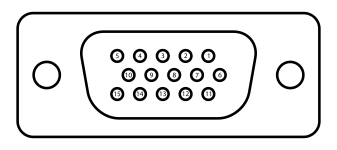
\includegraphics[height=2em]{slides/graphics-introduction/vga-pinout.pdf}
  \end{center}
  \begin{itemize}
  \item \textbf{Pixel}: Red, Green, Blue {\footnotesize(1, 2, 3)}, Ground returns {\footnotesize(6, 7, 8)}
  \item \textbf{Sync}: Hsync, Vsync {\footnotesize(13, 14)}
  \item \textbf{Side}: DDC SDA, DDC SCL {\footnotesize(12, 15)}
  \item \textbf{Power}: \(+5~V\) {\footnotesize(9)}, Ground {\footnotesize(10)}
  \end{itemize}
  \end{itemize}

\end{frame}

\begin{frame}{VGA display interface (illustrated)}
  \begin{center}
    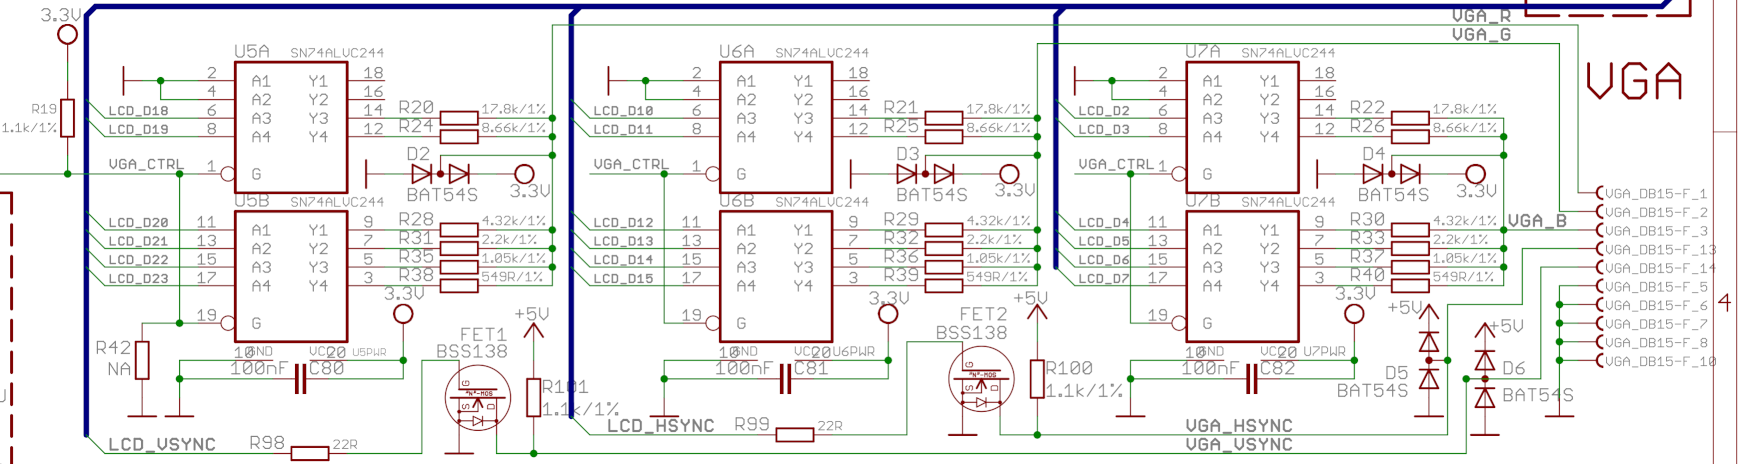
\includegraphics[width=\textwidth]{slides/graphics-introduction/a13-olinuxino-vga.png}
  \end{center}

  \begin{itemize}
  \item Very basic VGA encoder from parallel signals, DDC excluded
  \item Resistor ladder for analog-to-digital conversion\\
  \textit{using SN74ALVC244 voltage level shifters (\(1.8~V\) to \(3.3~V\)), clamping diodes}
  \item 6 most-significant bits only, 2 least-significant bits set to 0\\
  \textit{D0-D1, D8-D9 and D16-D17 are not routed}
  \end{itemize}
\end{frame}

\begin{frame}{DVI display interface}
  \begin{itemize}
  \item \textbf{Digital Visual Interface} (DVI), since 1999 (DDWG)
    \begin{itemize}
    \item \textbf{DVI-A}: Analog only, comparable to VGA
    \item \textbf{DVI-D}: Digital only, single-link (3 data lanes) or dual-link (6 data lanes)
    \item \textbf{DVI-I}: Both analog and digital supported, single-link or dual-link
    \item Digital serial link using \textbf{Transition-Minimized Differential Signaling} (TMDS)
    \item Dedicated \textbf{DDC} and \textbf{HPD} signals
    \item Using a subset or variation of the full \textbf{DVI-I connector} for signals:
    \end{itemize}
  \begin{center}
    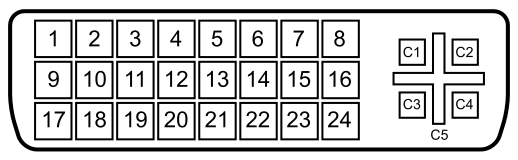
\includegraphics[height=2em]{slides/graphics-introduction/dvi-pinout.pdf}
  \end{center}
  \begin{itemize}
  \item \textbf{TMDS}: Data+ {\footnotesize(2, 5, 10, 13, 18, 21)}, Data- {\footnotesize(1, 4, 9, 12, 17, 20)}, Clock {\footnotesize(23, 24)}
  \item \textbf{Analog pixel}: Red, Green, Blue {\footnotesize(C1, C2, C3)}, Ground {\footnotesize(C5)}
  \item \textbf{Analog sync}: Hsync, Vsync {\footnotesize(C4, 8)}
  \item \textbf{Side}: DDC SDA, DDC SCL {\footnotesize(7, 6)}, HPD {\footnotesize(16)}
  \item \textbf{Power}: \(+5~V\) {\footnotesize(14)}, Ground {\footnotesize(15)}
  \end{itemize}
  \end{itemize}
\end{frame}

\begin{frame}{HDMI display interface}
  \begin{itemize}
  \item \textbf{High-Definition Multimedia Interface} (HDMI), since 2002 (HDMI Forum)
    \begin{itemize}
    \item Similar to \textbf{DVI-D}: no analog, 3 TMDS data lanes (R-G-B)
    \item Adding the use of AVI infoframes for meta-data and audio
    \item \textbf{High bandwidth} \((\leq 48~Gbit/s)\) (2.1) and clock speeds \((\leq 340~MHz)\)
    \item \textbf{Extra features}: Audio, CEC (1.2), HDR (1.3), 4K (1.4), Stereoscopy (1.4),\\8K-10K (2.1), DSC (2.1), HFR (\(120~Hz\)), per-frame HDR (2.1)
    \item Using a dedicated (and proprietary) \textbf{HDMI connector} for signals:
    \end{itemize}
  \begin{center}
    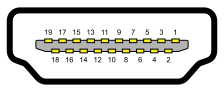
\includegraphics[height=2em]{slides/graphics-introduction/hdmi-pinout.pdf}
  \end{center}
  \begin{itemize}
  \item \textbf{TMDS}: Data+ {\footnotesize(1, 4, 7)}, Data- {\footnotesize(3, 6, 9)}, Clock {\footnotesize(10, 12)}
  \item \textbf{Side}: SDA, SCL {\footnotesize(16, 15)}, HPD {\footnotesize(19)}, CEC {\footnotesize(13)}
  \item \textbf{Power}: \(+5~V\) {\footnotesize(18)}, Ground {\footnotesize(17)}
  \end{itemize}
  \end{itemize}
\end{frame}

\begin{frame}{DP/eDP display interface}
  \begin{itemize}
  \item \textbf{DisplayPort} (DP), since 2008 (VESA)
    \begin{itemize}
    \item Digital serial link with 4 data lanes using \textbf{Low-Voltage Differential Signaling} (LVDS)
    or TMDS for DP Dual-Mode (DP++), compatible with DVI-D and HDMI
    \item Using \textbf{packets} for video/audio data and meta-data 
    \item Auxiliary channel encapsulating I2C DDC, CEC and more (e.g. USB)
    \item \textbf{High bandwidth} \((\leq 77.37~Gbit/s)\) (2.0)
    \item \textbf{Extra features}: Audio, CEC, HDR (1.4), 4K (1.3), Stereoscopy (1.2),\\8K (1.3-1.4),  10K-16K (2.0)
    \item \textbf{Multi-Stream Transport} (MST) to chain displays
    \item Using a dedicated (and proprietary) \textbf{DisplayPort connector} for signals:
    \end{itemize}
  \begin{center}
    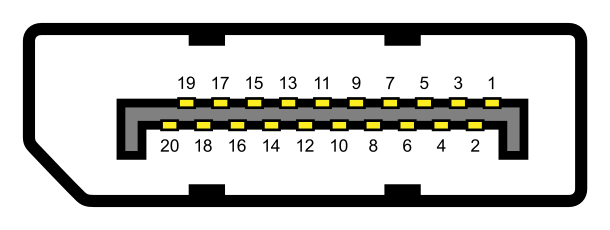
\includegraphics[height=2em]{slides/graphics-introduction/dp-pinout.pdf}
  \end{center}
  \begin{itemize}
  \item \textbf{LVDS/TMDS}: ML+ {\footnotesize(1, 4, 7, 10)}, ML- {\footnotesize(3, 6, 9, 12)}
  \item \textbf{Side}: AUX+ (15), AUX- (17), HPD (18)
  \item \textbf{Power}: \(+3.3~V\) {\footnotesize(20)}, Ground {\footnotesize(2, 5, 8, 11, 16)}
  \end{itemize}
  \item \textbf{Embedded DisplayPort} (eDP) for internal panels (without connector)
  \end{itemize}
\end{frame}

\begin{frame}{LVDS and DSI display interfaces}

% TODO split and add photo of custom LVDS connector as well as a DSI panel (librem 5 dvt?)

  \begin{itemize}
  \item \textbf{Low Voltage Differential Signaling} (LVDS)
    \begin{itemize}
    \item Generic digital serial link with clock and data signals using LVDS
    \item Only sends pixel data according to a pre-defined mode (no DDC, no packets)
    \item For internal panels, exposed with specific connectors
    \item Common for laptop panels
    \end{itemize}
  \item \textbf{Display Serial Interface} (DSI), since 2006 (MIPI)
    \begin{itemize}
    \item Digital serial link with clock and up to 4 data lanes using LVDS
    \item Using \textbf{packets} for video data and meta-data
    \item Commands for configuration can be issued with the \textbf{DSI Command Set} (DCS)\\
    \textit{Generic base with proprietary vendor-specific extensions}
    \item For internal panels, exposed with specific connectors
    \item Common for mobile devices' panels
    \end{itemize}
  \end{itemize}
\end{frame}

\begin{frame}{DPI display interface}
  \begin{itemize}
  \item \textbf{Display Parallel Interface} (DPI)
    \begin{itemize}
    \item Generic parallel digital interface, with 1 signal per color bit, clock and sync
    \item Exists with different numbers of bits: 24 (8-8-8), 18 (6-6-6) or 16 (5-6-5)\\
    \textit{Dithering is required when using 16 or 18 bits}
    \item Sends pixel data bits following mode timings
    \item Base signals: color data bits, vsync, hsync
    \item Extra signals: display enable (DE)
    \item Beware: sync and DE signals can be active-high or active-low
    \item For internal panels, requires many signals
    \end{itemize}
  \end{itemize}
\end{frame}

\begin{frame}{Bridges/transcoders}
  \begin{itemize}
  \item Not every display interface is supported by the hardware at hand
  \item Bridges or transcoders are used to translate from one interface to another
  \item They are composed of a decoder and an encoder (in a single package)
  \item Usually standalone and transparent, often only replicate timings\\
  \textit{but some can have a side-bus for configuration and fine-tuning}
  \item Example: VGA interfaces are usually bridged from digital interfaces nowadays
  \end{itemize}

  \begin{center}
  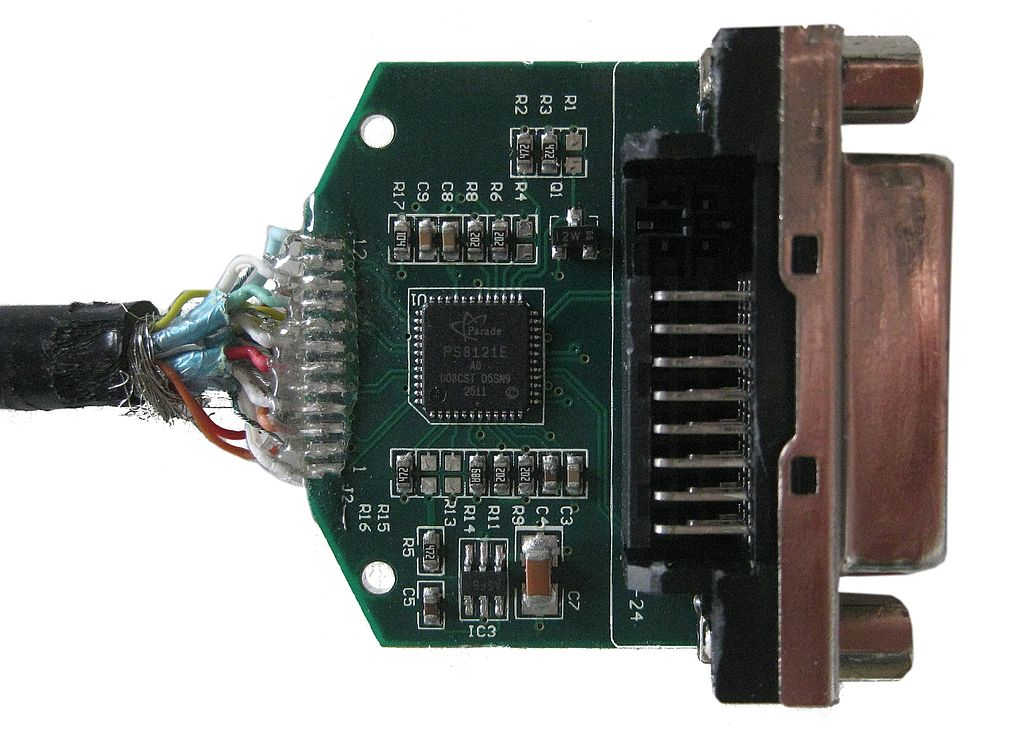
\includegraphics[height=6em]{slides/graphics-introduction/dp-dvi-bridge.jpg}\\
  \textit{\small A DP to DVI bridge}
  \end{center}
\end{frame}

\section{Software Aspects}

\subsection{Display Stack Overview}

\begin{frame}{System-agnostic overview: kernel}
  \begin{itemize}
  \item The kernel coordinates access to the hardware from userspace
  \item Handles register access, interrupts, etc
  \item Coordinates memory management with the rest of the system
  \item Exposes features to userspace through hardware-agnostic interfaces\\
  \textit{or at least, as much as possible}
  \item Three aspects are usually involved:
    \begin{itemize}
    \item \textbf{display}: from framebuffer to encoder
    \item \textbf{render}: GPU and/or 2D accelerators
    \item \textbf{input}: keyboard, mouse and other devices
    \end{itemize}
  \end{itemize}
\end{frame}

\begin{frame}{System-agnostic overview: display userspace}
  \begin{itemize}
  \item Userspace needs to provide a way for applications to show buffers
  \item Many applications need to show their buffers concurrently
  \item The \textbf{display server} is in charge of coordinating between applications:
    \begin{itemize}
    \item Part of the core of the system, privileged
    \item Applications (via libraries) contact the server to display pixel buffers
    \item Dispatches input events to the concerned applications
    \item Only the display server deals with the kernel display and input APIs
    \end{itemize}
  \item The \textbf{compositor} merges pixel buffers from applications into the final buffer
  \item The \textbf{window manager} defines stacking order, focus, decorations, etc
  \item Both can be part of the display server or distinct components
  \end{itemize}
\end{frame}

\begin{frame}{System-agnostic overview: display userspace (illustrated)}

  \begin{minipage}[t]{0.49\textwidth}
    \centering
    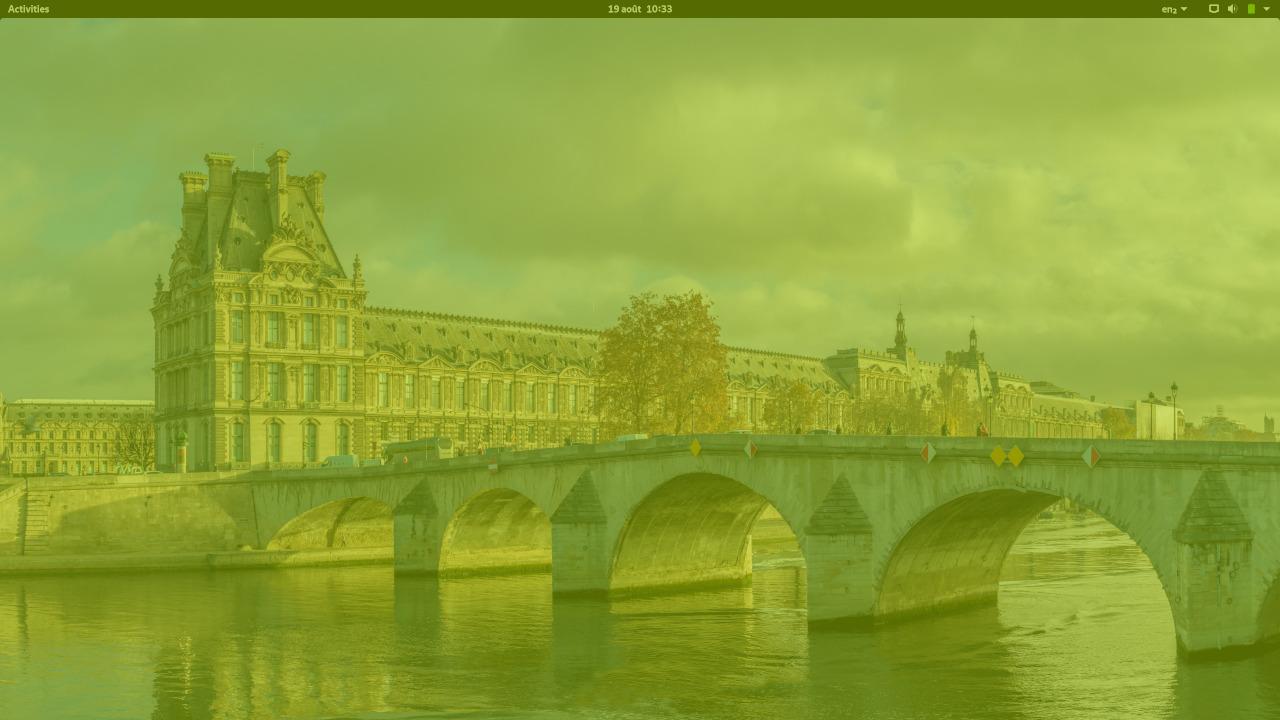
\includegraphics[height=7em]{slides/graphics-introduction/compositing-gnome-shell.jpg}\\
    \textit{\small GNOME-Shell (green) displaying the\\ top-bar and background}\\
    \vspace{0.5em}
    
\includegraphics[height=7em]{slides/graphics-introduction/compositing-gnome-terminal.jpg}\\
    \textit{\small GNOME-Terminal (green) with\\ window decorations (red)}
  \end{minipage}
  \hfill
  \begin{minipage}[t]{0.49\textwidth}
    \centering
    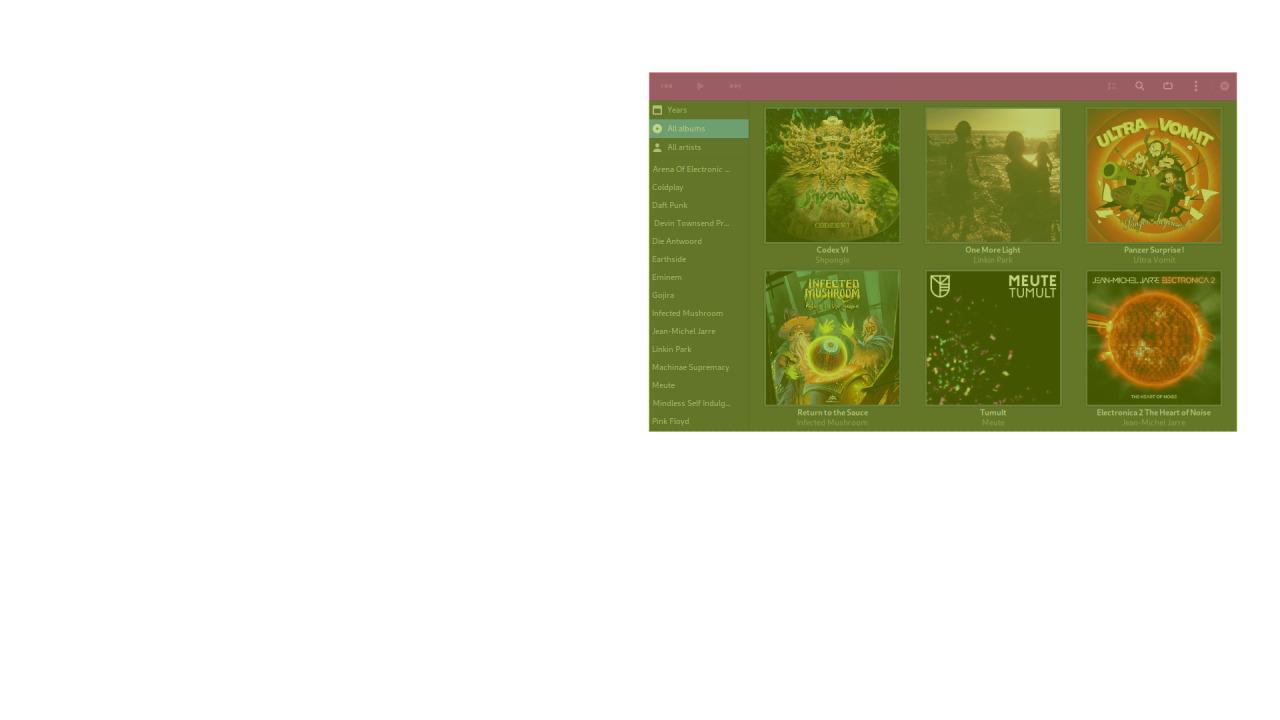
\includegraphics[height=7em]{slides/graphics-introduction/compositing-lollypop.jpg}\\
    \textit{\small Lollypop (green) with\\ window decorations (red)}\\
    \vspace{0.5em}
    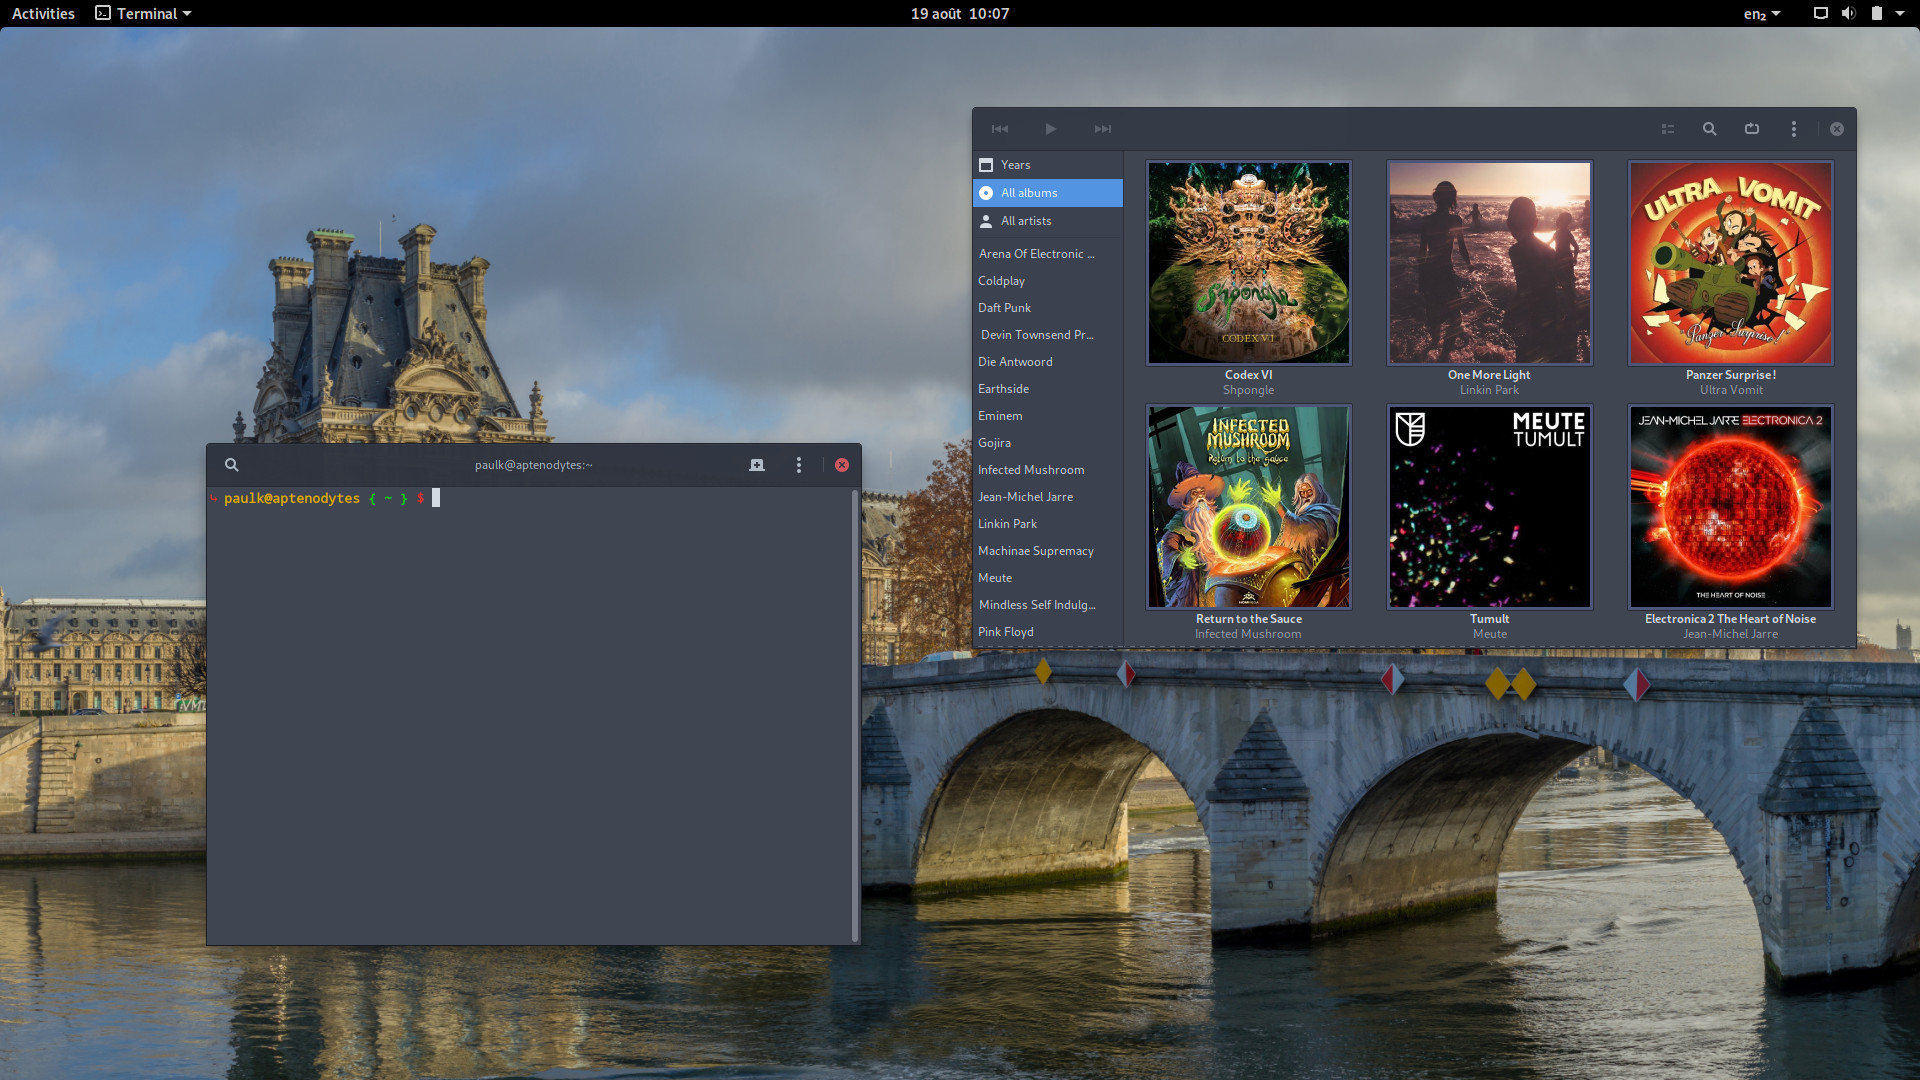
\includegraphics[height=7em]{slides/graphics-introduction/compositing-result.jpg}\\
    \textit{\small The composited result}
  \end{minipage}
\end{frame}

\begin{frame}{System-agnostic overview: render userspace}
  \begin{itemize}
  \item Graphics applications and libraries need to render visual elements
  \item Rendering can be a major \textbf{performance bottleneck}
  \item The system often provides \textbf{accelerated 2D primitives}:
    \begin{itemize}
    \item Either in the display server
    \item Either in dedicated libraries
    \end{itemize}
  \item Their implementation can take different forms:
    \begin{itemize}
    \item Using dedicated 2D hardware
    \item Using 3D hardware in 2D setups (\(z = 0\))
    \item Using specific efficient CPU instructions (SIMD)
    \item Using optimized generic algorithms
    \end{itemize}
  \item \textbf{3D rendering} comes with its own interfaces and libraries
  \item Usually with generic interfaces and hardware-specific implementations
  \end{itemize}
\end{frame}

\begin{frame}{System-agnostic overview (illustrated)}
  \begin{center}
  \includegraphics[width=\textwidth]{slides/graphics-introduction/agnostic-display-stack-overview.pdf}
  \end{center}
\end{frame}

\begin{frame}{Linux kernel overview}
  \begin{itemize}
  \item \textbf{Input} subsystem
    \begin{itemize}
    \item Supports devices such as mice, keyboards, joysticks, touchscreens
    \item Legacy (unused) interfaces for keyboard, mice
    \item Unified \textbf{evdev} event interface to simplify userspace
    \end{itemize}
  \item \textbf{Framebuffer device} (fbdev) subsystem
    \begin{itemize}
    \item \textbf{Legacy} interface for displaying pixel buffers on-screen
    \item Very limited pipeline configuration, no hotplug support
    \item Extended features added through driver-specific interfaces
    \end{itemize}
  \item \textbf{Direct Rendering Manager} (DRM) subsystem
    \begin{itemize}
    \item Unified display configuration interface: \textbf{Kernel Mode Setting} (KMS or DRM mode)
    \item Allows synchronizing changes together (DRM atomic)
    \item Exposes render devices through driver-specific interfaces (DRM render)\\
      \textit{Mostly for 3D rendering with GPUs, but a few 2D devices too}
    \item Provides memory management mechanisms (DRM GEM)
    \end{itemize}
  \end{itemize}

\end{frame}

\begin{frame}{Linux-compatible low-level userspace overview}
  \begin{itemize}
  \item \textbf{Input} low-level libraries
    \begin{itemize}
    \item \textbf{libevdev} (C): Wrapper for evdev interface system calls
    \item \textbf{libinput} (C): Input device management, abstraction and quirks, using libevdev
    \end{itemize}
  \item \textbf{Display/render} low-level interface library
    \begin{itemize}
    \item \textbf{libdrm} (C): Wrapper for DRM system calls
    \end{itemize}
  \item \textbf{2D render} low-level libraries
    \begin{itemize}
    \item \textbf{Pixman} (C): Optimized pixel-level operations
    \item \textbf{Cairo} (C): Optimized vector drawing (can use 3D)
    \item \textbf{Skia} (C): Optimized vector drawing from Google (can use 3D)
    \item \textbf{Clutter} (C++): Accelerated UI animation (using 3D)
    \end{itemize}
  \item \textbf{3D render} low-level libraries
    \begin{itemize}
    \item \textbf{Mesa 3D} (C): Reference free software OpenGL implementation
    \item \textbf{Proprietary vendor implementations} for specific hardware
    \end{itemize}
  \end{itemize}
\end{frame}

\begin{frame}{X Window overview}
  \begin{itemize}
  \item \textbf{X Window} overview
    \begin{itemize}
    \item \textbf{X Window/X11} is the historical (and \textbf{legacy}) \textbf{display protocol}
    \item Complemented by numerous protocol \textbf{extensions} for extra features
    \item \textbf{X.org} is the reference X11 server \textbf{implementation}
    \item Needs an external \textbf{window manager} to handle multiple applications
    \item \textbf{Composition} by the server or the window manager (Composite extension)
    \end{itemize}
  \end{itemize}
  \begin{minipage}[b]{0.8\textwidth}
  \begin{itemize}
  \item \textbf{Window manager} implementations examples
    \begin{itemize}
    \item \textbf{Mutter}: GNOME accelerated compositing window manager
    \item \textbf{i3}: Popular tiling window manager
    \item \textbf{Compiz}: Popular 3D-enabled compositing window manager
    \end{itemize}
  \item \textbf{Display client} libraries
    \begin{itemize}
    \item \textbf{Xlib} (C): The legacy X11 client-side protocol library helper
    \item \textbf{XCB} (C): The updated X11 client-side protocol library helper
    \item Integrated in most higher-level graphics-oriented libraries
    \end{itemize}
  \end{itemize}
  \end{minipage}
  \begin{minipage}[b]{0.15\textwidth}
  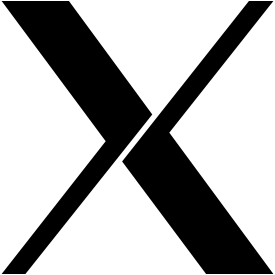
\includegraphics[width=\textwidth]{slides/graphics-introduction/x11-logo.pdf}
  \end{minipage}
\end{frame}

\begin{frame}{Wayland overview}
  \begin{itemize}
  \item \textbf{Wayland} overview
    \begin{itemize}
    \item Wayland is a \textbf{display protocol} (with a core and extensions), not an implementation
    \item Replaces X11 with a \textbf{less intrusive, more modern and minimal} paradigm
    \item Server implementation is in charge of \textbf{input, composition and window management}
    \item Window decorations can be drawn by the client or the server
    \end{itemize}
  \end{itemize}
  \begin{minipage}[b]{0.8\textwidth}
  \begin{itemize}
  \item \textbf{Wayland compositor} implementations examples
    \begin{itemize}
    \item Using the \textbf{libwayland-server} base protocol library
    \item \textbf{Weston/libweston}: Reference implementation
    \item \textbf{Sway/wlroots}: Tiling window manager and base library
    \item \textbf{Mutter}: GNOME compositor, expecting client-side decorations
    \end{itemize}
  \item \textbf{Display client} libraries
    \begin{itemize}
    \item Using the \textbf{libwayland-client} base protocol library
    \item Integrated in many higher-level graphics-oriented libraries
    \end{itemize}
  \end{itemize}
  \end{minipage}
  \begin{minipage}[b]{0.15\textwidth}
  
\includegraphics[width=\textwidth]{slides/graphics-introduction/wayland-logo.pdf}
  \end{minipage}
\end{frame}

\begin{frame}{High-level graphics libraries and desktop environments overview}
  \begin{minipage}[b]{0.09\textwidth}
  \centering
  
\includegraphics[width=\textwidth]{slides/graphics-introduction/gtk-logo.pdf}\\
  \vspace{3em}
  
\includegraphics[width=\textwidth]{slides/graphics-introduction/qt-logo.pdf}\\
  \vspace{3em}
  
\includegraphics[width=\textwidth]{slides/graphics-introduction/sdl-logo.png}\\
  \vspace{2em}
  \end{minipage}
  \hfill
  \begin{minipage}[b]{0.8\textwidth}
  \begin{itemize}
  \item Applications rarely to never use Wayland or X11 directly
  \item Drawing and managing a user interface is complex
  \item Widely-used high-level graphics libraries (aka toolkits)
    \begin{itemize}
    \item \textbf{GTK} (C): Widget-based UI toolkit, drawing helpers (GDK)
    \item \textbf{Qt} (C++): Widget-based UI toolkit, wide framework
    \item \textbf{EFL} (C): Lightweight UI and application library
    \item \textbf{SDL} (C): Drawing-oriented graphics library (used in games)
    \end{itemize}
  \item A desktop environment groups related libraries and components\\
  \textit{gives a consistent look and feel across the system}
  \item \textbf{Desktop environment} examples
    \begin{itemize}
    \item \textbf{GNOME}: Using GTK, GNOME-Shell desktop
    \item \textbf{KDE}: Using Qt, Plasma desktop
    \item \textbf{Xfce}: Using GTK, lightweight
    \item \textbf{Enlightenment}: Using EFL
    \end{itemize}
  \end{itemize}
  \vfill~
  \end{minipage}
  \begin{minipage}[b]{0.09\textwidth}
  \centering
  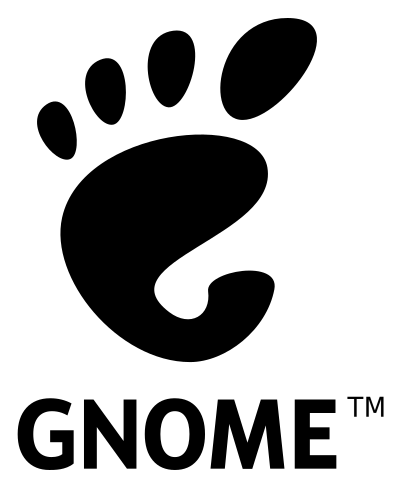
\includegraphics[width=\textwidth]{slides/graphics-introduction/gnome-logo.pdf}\\
  \vspace{1em}
  
\includegraphics[width=\textwidth]{slides/graphics-introduction/kde-logo.pdf}\\
  \vspace{1em}
  
\includegraphics[width=\textwidth]{slides/graphics-introduction/xfce-logo.pdf}\\
  \vspace{0.5em}
  
\includegraphics[width=\textwidth]{slides/graphics-introduction/enlightenment-logo.pdf}
  \end{minipage}
\end{frame}

\subsection{Kernel Aspects}

\begin{frame}{Linux TTY subsystem introduction}
  \begin{itemize}
  \item The \textbf{TTY} subsystem handles teletypewriters to send/receive characters
  \item Source code located at \code{drivers/tty} in Linux
  \item Supports physical instances (e.g. UART, RS-232) and virtual ones
  \item Virtual terminals/consoles (VTs/VCs) associate a distinct keyboard and display
    \begin{itemize}
    \item Many VTs are created by Linux, available under \code{/dev/tty*}
    \item Only a single VT is active at a time, switched with \code{Ctrl + Alt + Fi}
    \item Display grabbed using \textbf{fbcon} from the \textbf{fbdev} subsystem
    \item Keyboard grabbed using the \textbf{input} subsystem
    \item Can be used to show kernel messages (\code{console=tty1} in the cmdline)
    \item Every program runs under a controlling tty (given by the \code{tty} command)
    \end{itemize}
  \item Pseudo-terminals also exist, for software-based I/O only
    \begin{itemize}
    \item Created by programs (e.g. terminal emulator) under \code{/dev/pts/*}
    \item Unrelated to graphics topics
    \end{itemize}
  \end{itemize}
\end{frame}

\begin{frame}[fragile]{Virtual terminals and graphics}
  \begin{itemize}
  \item With VTs, the kernel is \textbf{already using} the display and keyboard!
  \item Display servers need to switch to \textbf{graphics mode} to release the display:
  \begin{minted}[fontsize=\small]{console}
ret = ioctl(tty_fd, KDSETMODE, KD_GRAPHICS);
  \end{minted}
  \item And disable \textbf{keyboard support} on the standard input:
  \begin{minted}[fontsize=\small]{console}
ret = ioctl(tty_fd, KDSKBMODE, K_OFF);
  \end{minted}
  \item The display device can then be used \textbf{exclusively}
  \item Input is no longer interpreted (e.g. \code{Ctrl-C} is ignored)
  \item Graphics and keyboard mode must be restored when leaving to keep the VT usable
  \item Current modes can be queried with:
  \begin{minted}[fontsize=\small]{console}
short mode, kbmode;
ret = ioctl(tty_fd, KDGETMODE, &mode);
ret = ioctl(tty_fd, KDGKBMODE, &kbmode);
  \end{minted}
  \item More details on the \code{console_ioctl} man page
  \end{itemize}
\end{frame}

\begin{frame}[fragile]{Virtual terminals switching and graphics}
  \begin{itemize}
  \item However, the user might still want to switch VTs!
  \item So the display device must be \textbf{released/reacquired} for VT switching
  \item Unix signals are used to notify the application, configured with:
  \begin{minted}[fontsize=\small]{console}
struct vt_mode vt_mode;
vt_mode.mode = VT_PROCESS;
vt_mode.relsig = SIGUSR1;
vt_mode.acqsig = SIGUSR2;
ret = ioctl(tty_fd, VT_SETMODE, &vt_mode);
  \end{minted}
  \item VT switching must be acknowledged for the other VT to take over:
  \begin{minted}[fontsize=\small]{console}
ret = ioctl(tty_fd, VT_RELDISP, VT_ACKACQ); /* when entering VT */
ret = ioctl(tty_fd, VT_RELDISP, 1); /* when leaving VT */
  \end{minted}
  \item Failure to acknowledge will cause a \textbf{system hang}
  \end{itemize}
\end{frame}

% XXX: Add list of relevant code in wayland/xorg?

\subsection{Userspace Aspects}
